
%!TEX option = --shell-escape

\documentclass[9pt, xcolor={svgnames, x11names},professionalfonts]{beamer}


\usepackage{xcolor}
\usepackage{cancel}
\usepackage{bm}
\usepackage{graphicx}
\usepackage{hyperref}
\usepackage{adjustbox}
\hypersetup{colorlinks, allcolors=.,urlcolor=structure}
\usepackage{booktabs}  % for top and bottom spacing in table cells, \addlinespace
\usepackage[x11names, svgnames]{xcolor} % for colors in handouts, auto loaded in Beamer?
\usepackage{tikz}
\usetikzlibrary{arrows.meta, math, calc, shadows,bending}
\usetikzlibrary{decorations.markings, decorations.fractals, decorations.text} % for chain, etc.
\usetikzlibrary{intersections}
\usepackage{pgfmath}
\usepackage{ifthen}
\usepgfmodule{oo}
\usetikzlibrary{shadings}
% \usetikzlibrary{decorations.shapes}
\usepackage[many]{tcolorbox}
\tcbuselibrary{skins} % for image boxes
\usepackage[absolute,overlay,showboxes]{textpos}
% \usepackage{textpos}
% \textblockorigin{0.0cm}{0.0cm}  %start all at upper left corner
\TPshowboxesfalse

\newcommand\lb{\linebreak}
\newcommand\Ra{\Rightarrow}
\newcommand\cd{\!\cdot\!}
\newcommand\x{\!\times\!}
\newcommand\pars{\par\smallskip}
\newcommand\parm{\par\medskip}
\newcommand\parb{\par\bigskip}
\renewcommand{\deg}{^\circ}

% counter for resuming enumerated list numbers
\newcounter{resumeenumi}
\newcommand{\suspend}{\setcounter{resumeenumi}{\theenumi}}
\newcommand{\resume}{\setcounter{enumi}{\theresumeenumi}}



% https://tex.stackexchange.com/questions/33703/extract-x-y-coordinate-of-an-arbitrary-point-in-tikz
\makeatletter
\providecommand{\gettikzxy}[3]{%
	\tikz@scan@one@point\pgfutil@firstofone#1\relax
	\edef#2{\the\pgf@x}%
	\edef#3{\the\pgf@y}%
}
\makeatother

\makeatletter
\newcommand{\verbatimfont}[1]{\def\verbatim@font{#1}}%
\makeatother

%%%%%%%%%%%%%%%%%%%%%%%%%%%%%%%%%%%%%%%%%%%%%%%%%%%%%%%%%%%%%%%%%%%%%%%%%%%%%%%%


% \newcommand{\tb}[4][0.8]{
% 	\begin{textblock*}{#1}(#2, #3)
% 		\raggedright
% 		#4
% 	\end{textblock*}
% }

% \def\tb

\newtcolorbox{statsbox}[2][] { 
  colback=white,
  colbacktitle=structure,
  colframe=structure,
  coltitle=white,  
  top=0.25cm,
	bottom=0.125cm,
	left=0mm,
	right=0mm,
  % fonttitle=\itshape\rmfamily,
  halign=flush left, 
  enhanced,
  drop fuzzy shadow,
  attach boxed title to top left={xshift=3.5mm, yshift=-2mm},
  title={#2}, #1}
\newtcolorbox{redbox}{colback=white, colframe=structure, enhanced, drop fuzzy shadow}
\newtcolorbox{titledbox}[1]{colback=white,colframe=structure,title={#1}}
\newtcbox{\tcb}[1][]{colback=white,boxsep=0pt,top=0.5cm,bottom=0.5cm,left=0.5cm,
		right=0.5cm, colframe=structure,  enhanced, drop fuzzy shadow, #1}
\newtcbox{\tcbfig}[1][1]{colback=white,boxsep=0pt,top=0.5cm,bottom=0.5cm,left=0.5cm,
		right=0.5cm, colframe=structure,  enhanced, drop fuzzy shadow, #1}
% tcb title
\newtcbox{\tcbt}[2][]{colback=white,boxsep=0pt,top=5pt,bottom=5pt,left=5pt,
		right=5pt, colframe=structure, enhanced, drop fuzzy shadow,  title={#2}, #1}
% tcb left title
\newtcbox{\tcbtl}[2][]{ colback=white,
  colbacktitle=structure,
  colframe=structure,
  coltitle=white,  
  top=0.25cm,
	bottom=0.125cm,
	left=0mm,
	right=0mm,
  % fonttitle=\bfseries,
  halign=flush left, 
  enhanced,
  drop fuzzy shadow,
  attach boxed title to top left={xshift=3.5mm, yshift=-2mm}, 
	title={#2}, #1}

\newtcbtheorem{myexam}{Example}%
{
	enhanced,
	colback=white,
	colframe=structure,
	% fonttitle=\bfseries,
	fonttitle=\itshape\rmfamily,
	drop fuzzy shadow,
	%description font=\mdseries\itshape,
	attach boxed title to top left={yshift=-2mm, xshift=5mm},
	colbacktitle=structure
	}{exam}% then \pageref{exer:theoexample} references the theo

% \newcommand{\myexample}[2][red]{
% 	% \tcb\tcbset{theostyle/.style={colframe=red,colbacktitle=yellow}}
% 	\begin{myexam}{}{}
% 		#2
% 	\end{myexam}
% 	% \tcbset{colframe=structure,colbacktitle=structure}
% }

\newtcbtheorem{myexer}{Exercise}%
{
	enhanced,
	colback=white,
	colframe=structure,
	% fonttitle=\bfseries,
	drop fuzzy shadow,
	fonttitle=\itshape\rmfamily,
	% description font=\mdseries\itshape,
	attach boxed title to top left={yshift=-2mm, xshift=5mm},
	colbacktitle=structure
	}{exer}



\newcommand{\mini}[2][0.8]{
	\begin{minipage}[c]{#1\columnwidth}
		\raggedright
		#2
	\end{minipage}
}
\newcommand{\minit}[2][0.8]{
	\begin{minipage}[t]{#1\columnwidth}
		% \raggedright
		#2
	\end{minipage}
}

% centered minipage with text \raggedright
%\cmini[width]{content}
\newcommand{\cmini}[2][0.8]{
	\begin{center}
		\begin{minipage}{#1\columnwidth}
			\raggedright
			#2
		\end{minipage}
	\end{center}
}

\newcommand{\fig}[2][1]{% scaled graphic
	\includegraphics[scale=#1]{#2}
}

% centred framed box black border
%\cbox[width]{content}
\newcommand{\cbox}[2][1]{% framed centered color box
	\setlength\fboxsep{5mm}
	\setlength\fboxrule{.2 mm}
	\begin{center}
		\fcolorbox{black}{white}{
			\vspace{-0.5cm}
			\begin{minipage}{#1\columnwidth}
				\raggedright
				#2
			\end{minipage}
		}
	\end{center}
	\setlength\fboxsep{0cm}
}

\newcommand{\ccbox}[4][1]{% framed centered color box
	\setlength\fboxsep{5mm}
	\setlength\fboxrule{.2 mm}
	\begin{center}
		\fcolorbox{#2}{#3}{
			% \vspace{-0.5cm}
			\begin{minipage}{#1\columnwidth}
				\vspace{-0.25cm}
				\raggedright				
				#4
				\vspace{-0.325cm}
			\end{minipage}
		}
	\end{center}
	\setlength\fboxsep{0cm}
}

\newcommand{\cfig}[2][1]{% centred, scaled graphic
	\begin{center}
		% \fcolorbox{structure}{white}{
		\tcbincludegraphics{
			\includegraphics[scale=#1]{#2}
		}
	\end{center}
}

% figure with tight border for photos
% \cfigb[saitMaroon]{borderwidth with unit}{scale}{image}
\newcommand{\stcsfig}[2][1]{
	% \usepackage{adjustbox}
	% \setlength{\fboxrule}{1pt}
	\begin{center}
		\tcbincludegraphics[width=#1\textwidth, boxrule=2pt, top=-3pt, right=-3pt, left=-3pt, bottom=-3pt,colframe=structure, sharp corners, enhanced, drop fuzzy shadow]{#2}
	\end{center}
}






 \definecolor{saitPurple}{RGB}{112,40,119}
 \definecolor{statsMaroon}{rgb}{0.55, 0, 0}
 \definecolor{saitMaroon}{rgb}{0.55, 0, 0}
 \definecolor{saitRed}{RGB}{224,38,37}
 \definecolor{saitBlue}{rgb}{0, 0.59, 0.85}
 \definecolor{statsDeepBlue}{RGB}{0, 99, 167}
 \definecolor{saitDeepBlue}{RGB}{0, 99, 167}
 \definecolor{LightGrey}{RGB}{200,200,200}
%  \definecolor{boxBG}{RGB}{236, 227, 227}
%  \definecolor{boxBG}{RGB}{242, 233, 223}
% !TEX root = ../Beamer/statikz/statikz.tex

% \Channel[rotate=0]{coordinate}{draw}{fill}{scale}{lineWidth}
\newcommand{\Channel}[6][0]{
	\def\rotate{#1};
	\def\mid{#2}
	\def\lfill{#3}
	\def\lstroke{#4}
	\def\scale{#5};
	\def\lineWidth{#6};

	\begin{scope}[rounded corners=1pt, scale=\scale, rotate=\rotate]
		\filldraw[draw=\lstroke, fill=\lfill, line width=\lineWidth pt] ($(\mid) + (0,-3) $) -- ++(1.7,0) arc(0:85:0.25) -- ($ (\mid)+(0.4,-2.6) $) -- ($ (\mid)+(0.4,2.6) $) -- +(8.13:1.097)arc(-81.87:0:0.25) -- ($ (\mid)+(0,3) $)  -- cycle;
	\end{scope}
}

\newcommand{\Couple}[5][1]{
	\def\positive{#1};
	\def\lpin{#2}	
	\def\ldraw{#3}
	\def\diam{#4}
	\def\lwidth{#5}
	
	\begin{scope}[line cap = round]
		\ifthenelse{\equal{\positive}{1}}
			{
				\draw[line width=\lwidth mm, \ldraw, -{Latex[length=\lwidth*12, bend]}] ($ (\lpin)+(-150:\diam) $) arc (-150:165:\diam);
				% \draw[-latex, \ldraw, line width=\lwidth mm] ($ (\lpin)+(150:\diam) $) --+ (240:\lwidth/5);
			}
			{
				\draw[line width=\lwidth mm, \ldraw, -{Latex[length=\lwidth*12, bend]}] ($ (\lpin)+(150:\diam) $) arc (150:-165:\diam);
				% \draw[-latex, \ldraw, line width=\lwidth mm] ($ (\lpin)+(-140:\diam) $) --+ (120:\lwidth/5 );
			}
		
	\end{scope}
}
\newcommand{\DL}[9][1]{
  \def\forcedown{#1} % defaults to 1, force is downward
  \def\tl{#2} % top left, a coordinate
  \def\tr{#3} % top right. a coordinate
  \def\b{#4} % anywhere along the baseline (before any rotation), a coordinate 
  \def\lfill{#5} % background fill color
  \def\stroke{#6} % drawing color
  \def\spaces{#7} % number of spaces between arrows 
  \def\llinewidth{#8}
  \def\tiplength{#9}

  \gettikzxy{(\tl)}{\tlx}{\tly}
	\gettikzxy{(\tr)}{\trx}{\try}
	\gettikzxy{(\b)}{\bx}{\by}
  \pgfmathparse{abs(\try-\by)} \let\rlength\pgfmathresult
  \pgfmathparse{abs(\tly-\by)} \let\llength\pgfmathresult

  \fill[\lfill] (\tlx, \tly)--(\trx, \try)--(\trx, \by)--(\tlx, \by);
  \draw[\stroke, line cap = round, line width = \llinewidth mm] (\tl)--(\tr);
  
  % no empty lines in \tikzmath!
  \tikzmath{
    % Calculate the width of the load, and the spacing between arrows
    % Also, calculate the difference in length between adjacent arrows.
    \dx = \trx - \tlx; % width of dist load
    \dx = \dx / \spaces; % space between arrows
    \dy = \try - \tly; % difference between two load values
    \dy = \dy / \spaces; % difference between arrow-line lengths
    %    
    if \forcedown == 1 then {       
			for \i in {0,...,\spaces} {	
        \starty = \tly+\i*\dy;
        \length = \starty-\by;
        % in \tikzmath, drawing commands are enclosed in { }; 
        {
          \begin{scope}          
            \clip (\tlx,\tly) -- (\trx, \try) -- (\trx,\by) --(\tlx,\by);
            \draw[\stroke, line width = \llinewidth mm, -{Latex[length=\tiplength]}](\tlx+\i*\dx, \starty pt)-- +(270: \length pt);
          \end{scope}
        };
			};
    } else {
      for \i in {0,...,\spaces} {	
        \starty = \tly+\i*\dy;
        \length = \starty-\by;			
				{
          \begin{scope}          
            \clip (\tlx,\tly) -- (\trx, \try) -- (\trx,\by) --(\tlx,\by);
            \draw[\stroke, line width = \llinewidth mm, {Latex[length=\tiplength]}-](\tlx+\i*\dx, \starty pt)-- +(270: \length pt);
          \end{scope}          
        };
			};      
    };
    if \forcedown == 1 then {
      if \rlength > \tiplength then {
        {\draw[\stroke, line width = \llinewidth mm, -{Latex[length=\tiplength]}] (\trx, \try)--(\trx, \by);};
      } else {
         {\draw[\stroke, line width = \llinewidth mm] (\trx, \try)--(\trx, \by);};
      };    
      if \llength > \tiplength then {
        {\draw[\stroke, line width = \llinewidth mm, -{Latex[length=\tiplength]}] (\tlx, \tly)--(\tlx, \by);};
      } else {
        {\draw[\stroke, line width = \llinewidth mm] (\tlx, \tly)--(\tlx, \by);};
      };
    } else {
      if \rlength > \tiplength then {
        {\draw[\stroke, line width = \llinewidth mm, {Latex[length=\tiplength]}-] (\trx, \try)--(\trx, \by);};
      } else {
        {\draw[\stroke, line width = \llinewidth mm] (\trx, \try)--(\trx, \by);};
      };    
      if \llength > \tiplength then {
        {\draw[\stroke, line width = \llinewidth mm, {Latex[length=\tiplength]}-] (\tlx, \tly)--(\tlx, \by);};
      } else {
        {\draw[\stroke, line width = \llinewidth mm] (\tlx, \tly)--(\tlx, \by);};
      };
    };    
  } % \end tikzmath environment
} % end of \DL definition
\input{../../includes/DLdown.tex}
% !TEX root = ../Beamer/02ForceVectors/02ForceVectors.tex


\newcommand{\EyeBolt}[6][0]{
	\def\lrotate{#1};
	\def\lpin{#2}
	\def\lfill{#3}
	\def\ldraw{#4}
	\def\lscale{#5}
	\def\lwidth{#6}
	%\def\h{1.5}
	\def\r{0.3}
	\begin{scope}[scale=\lscale, rotate=\lrotate]
		\filldraw[draw=\ldraw, fill=\lfill, line width=\lwidth pt] ($(\lpin) + (-0.7,-1.25)$) arc(180:90:.2) -- ++(0.05,0)arc(-90:0:0.2) -- ++(0.05,0.65)arc(225:-45:0.28284)-- ++(0.05,-.65)arc(180:270:.2)-- ++(0.05,0)arc(90:0:0.2) -- cycle;
		\fill[outer color=\lfill, inner color=black, line width = 0] (\lpin) circle (2.25mm);
		\filldraw[fill=white, draw=\ldraw, line width = \lwidth pt] (\lpin) circle (1.25mm);

		\begin{scope}[even odd rule]
			\fill[\lfill] (\lpin) circle (2.5mm)
			(\lpin) circle (2.125mm);
		\end{scope}

		\filldraw[rounded corners=\lscale pt, draw=\ldraw, fill=\lfill, line width=\lwidth pt] ($ (\lpin) - (1,1.5) $) rectangle +(2,0.25);
	\end{scope}
}

% !TEX root = ../../Beamer/statikz/statikz.tex


\newcommand{\EyeConnection}[6][0]{
	\def\lrotate{#1};
	\def\lpin{#2}
	\def\lfill{#3}
	\def\ldraw{#4}
	\def\lscale{#5}
	\def\lwidth{#6}
	\def\h{1}
	\def\r{0.3}
	\begin{scope}[scale=\lscale, rotate=\lrotate]
		\filldraw[draw=\ldraw, fill=\lfill, line width=\lwidth pt] ($(\lpin) + (0.201*\h+1.0353*\r ,-0.75*\h)$) -- ++(105: 0.77646*\h+0.26795*\r) arc (15:165:\r) -- ++(-105:0.77646*\h+0.26795*\r) -- cycle;

		\fill[outer color=\lfill, middle color=red, inner color=black, line width = \lwidth pt] (\lpin) circle (2.5mm);
		\filldraw[fill=white, draw=\ldraw, line width = \lwidth pt] (\lpin) circle (1.25mm);

		\filldraw[rounded corners=\lscale pt, draw=\ldraw, fill=\lfill, line width=\lwidth pt] ($ (\lpin) - (1,1) $) rectangle +(2,0.25);
	\end{scope}
}

%\Member{startpt}{endpt}{outer fill color}{inner fill color}{stroke}{height}{radius}{linewidth}
\providecommand{\Member}[8]{
  % name the points
  \coordinate(start) at (#1);
  \coordinate(end) at (#2);
  \edef\ofill{#3}%
  \edef\ifill{#4}%
  \edef\stroke{#5}%
  \edef\height{#6} % cm
  \edef\radius{#7} % cm
  \edef\linewidth{#8} % mm

  \coordinate(delta) at ($ (end)-(start) $);
  \gettikzxy{(delta)}{\dx}{\dy}
  \gettikzxy{(start)}{\sx}{\sy}
  \pgfmathparse{veclen(\dx, \dy)} \let\length\pgfmathresult

  \pgfmathparse{\dx==0}%
  % \ifnum low-level TeX for integers
  \ifnum\pgfmathresult=1 % \dx == 0
    \pgfmathsetmacro{\rot}{\dy > 0 ? 90 : -90}
  \else
    \pgfmathsetmacro{\rot}{\dx > 0 ? atan(\dy / \dx) : 180 + atan(\dy / \dx)}
  \fi

  
   
  \shadedraw[transform canvas = { rotate around = {\rot:(\sx,\sy)}}, line width = \linewidth, rounded corners = \radius mm, top color = \ofill, bottom color = \ofill, middle color = \ifill, draw = \stroke] ($ (start)+(-0.5*\height, 0.5*\height) $) -- ++(\height cm +\length pt, 0 ) -- ++(0, -\height) -- ++ (-\height cm -\length pt, 0) -- cycle;


  \shadedraw[ball color = \ofill!50!\ifill, draw = \stroke] (start) circle (\height/8);
  \shadedraw[ball color = \ofill!50!\ifill, draw = \stroke] (end) circle (\height/8);
  %  \pgfresetboundingbox

  
  


}

%\Member{startpt}{endpt}{outer fill color}{inner fill color}{stroke}{height}{radius}{linewidth}
\providecommand{\Mem}[8]{
  % name the points
  \coordinate(start) at (#1);
  \coordinate(end) at (#2);
  \edef\ofill{#3}%
  \edef\ifill{#4}%
  \edef\stroke{#5}%
  \edef\height{#6} % cm
  \edef\radius{#7} % cm
  \edef\linewidth{#8} % mm

  \coordinate(delta) at ($ (end)-(start) $);
  \gettikzxy{(delta)}{\dx}{\dy}
  \gettikzxy{(start)}{\sx}{\sy}
  \gettikzxy{(end)}{\ex}{\ey}
  \pgfmathparse{veclen(\dx, \dy)} \let\length\pgfmathresult

  \pgfmathparse{\dx==0}%
  % \ifnum low-level TeX for integers
  \ifnum\pgfmathresult=1 % \dx == 0
    \pgfmathsetmacro{\rot}{\dy > 0 ? 90 : -90}
  \else
    \pgfmathsetmacro{\rot}{\dx > 0 ? atan(\dy / \dx) : 180 + atan(\dy / \dx)}
  \fi
  \pgfmathparse{\dy==0}%
  % \ifnum\pgfmathresult=1 % \dx == 0
  %   \pgfmathsetmacro{\rot}{\dy > 0 ? 0 : 180}
  % \fi

  \pgfdeclareverticalshading{myshading}{\length pt}{
    color(0)=(\ofill); color(0.5*\length pt-0.5*\height cm)=(\ofill); color(0.5*\length pt)=(\ifill); color(0.5*\length pt+0.5*\height cm)=(\ofill); color(\length pt)=(\ofill)
  }

  
  \begin{scope}[shading=myshading] 
    \shadedraw[rotate around = {\rot:(\sx,\sy)}, line width = \linewidth mm, rounded corners = \radius cm, draw = \stroke, shading angle=\rot] ($ (\sx,\sy)+(-0.5*\height cm, 0.5*\height cm) $) -- ++(\height cm +\length pt, 0 ) -- ++(0, -\height cm) -- ++ (-\height cm -\length pt, 0) -- cycle;
    %  \node[below] at (\sx, \sy) {\length};
  \end{scope}

%  \pgfresetboundingbox
  \shadedraw[ball color = \ofill!50!\ifill, draw = \stroke] (start) circle (\height/8);
  \shadedraw[ball color = \ofill!50!\ifill, draw = \stroke] (end) circle (\height/8);
  

  % \node at (\ex,\ey+1cm){$\rot\deg$};
  


}

%\Member{startpt}{endpt}{outer fill color}{inner fill color}{stroke}{height}{radius}{linewidth}
\providecommand{\Meme}[8]{
  \coordinate(start) at (#1);
  \coordinate(end) at (#2);
  \edef\ofill{#3}%
  \edef\ifill{#4}%
  \edef\stroke{#5}%
  \edef\height{#6} % cm
  \edef\radius{#7} % cm, should be half \height or less
  \edef\linewidth{#8} % mm

  


  \coordinate(delta) at ($ (end)-(start) $);
  \gettikzxy{(delta)}{\dx}{\dy}
  \gettikzxy{(start)}{\sx}{\sy}
  \gettikzxy{(end)}{\ex}{\ey}
  \pgfmathparse{veclen(\dx, \dy)} \let\length\pgfmathresult
  \pgfmathparse{\height*28.435} \let\heightpt\pgfmathresult
  \pgfmathparse{\heightpt/\length} \let\ratio\pgfmathresult
  \pgfmathparse{1/\ratio} \let\inverse\pgfmathresult
  

  \pgfmathparse{\dx==0}%
  % \ifnum low-level TeX for integers
  \ifnum\pgfmathresult=1 % \dx == 0
    \pgfmathsetmacro{\rot}{\dy > 0 ? 90 : -90}
  \else
    \pgfmathsetmacro{\rot}{\dx > 0 ? atan(\dy / \dx) : 180 + atan(\dy / \dx)}
  \fi

  \pgfmathparse{round(mod(abs(\rot),90))} \let\tmp\pgfmathresult
  \pgfmathsetmacro{\rotmod}{\tmp>45?90-\tmp:\tmp}
  \pgfmathparse{(0.007*\rotmod-0.315)/45+1.017} \let\rotfudge\pgfmathresult

  % \pgfmathparse{mod(abs(\rot),90)} \let\moded\pgfmathresult
  % \ifthenelse{\moded>45}{
  %   \pgfmathparse{90-\moded} \let\rotmod\pgfmathresult    
  % }{
  %   \pgfmathparse{div(\moded,1)} \let\rotmod\pgfmathresult   
  % }


  
  \pgfmathparse{1+3.62/(1+(\inverse/0.714)^1.69)} \let\fudge\pgfmathresult
  \pgfmathparse{50*(1-\ratio)*\fudge*\rotfudge} \let\colorstop\pgfmathresult
  \pgfmathparse{(100-\colorstop)} \let\colorstoptwo\pgfmathresult

  \pgfdeclareverticalshading{myshade}{100bp}{%
					color(0bp)=(\ofill);
					% color(\colorstop bp)=(\ofill);
					color(\colorstop bp)=(\ofill);
					color(50 bp)=(\ifill);
					color(\colorstoptwo bp)=(\ofill);
					color(100bp)=(\ofill)}

  % \tikzset{shading=myshade}

  \begin{scope}[rotate around = {\rot:(start)}, rounded corners = \radius cm, shading angle=\rot]
    \begin{scope} 
      \path[clip]($ (start)+(-0.5*\height, 0.5*\height cm) $) rectangle +(\length pt+\height cm, -\height);
      \shade[shading=myshade] ($ (start)+(-0.5*\height, 0.5*\length pt) $) rectangle +(\length pt+\height cm, -\length pt);
    \end{scope}
  \draw[line width=\linewidth, \stroke] ($ (start)+(-0.5*\height, 0.5*\height cm) $) rectangle +(\length pt+\height cm, -\height);

  % \shadedraw[top color=\ofill, bottom color=\ofill, middle color=\ifill, rotate around = {\rot:(start)}, draw=\stroke, rounded corners = \radius cm, , shading angle=\rot] ($ (start)+(-0.5*\height cm, 0.5*\length pt) $) rectangle +(\length pt+\height cm, -\length pt);
  \end{scope}

  % \pgfresetboundingbox


  % \node[orange] at (0,-1) {rot: \rot};  
  % \node[orange] at (0,-1.5) {rotmod: \rotmod};  
  % \node[orange] at (0,-2) {rotfudge: \rotfudge};  
  % \node[orange] at (-2,-1) {stop2: \colorstoptwo};  
  % \node[orange] at (-2,-1.5) {l/h: \inverse};  
  % \node[orange] at (-2,-2) {fudge: \fudge};  

 
  
  \shade[ball color=\ofill] (start) circle (\height/4);
  \shade[ball color=\ofill] (end) circle (\height/4);

  % \draw(current bounding box.south west) rectangle (current bounding box.north east);


}

\newcommand{\PC}[6][0]{%
  \edef\lrotate{#1}%
  \edef\lpin{#2}%
  \edef\lfill{#3}%
  \edef\ldraw{#4}%
  \edef\lscale{#5}%
  \edef\lwidth{#6}%
  \edef\h{1}%
  \edef\r{0.3}%
  \begin{scope}[scale=\lscale, rotate=\lrotate]
	\filldraw[draw=\ldraw, fill=\lfill, line width=\lwidth mm] ($ (\lpin) + (0.201*\h+1.0353*\r ,-0.75*\h) $) -- ++(105: 0.77646*\h+0.26795*\r) arc (15:165:\r) -- ++(-105:0.77646*\h+0.26795*\r) -- cycle;

	\shadedraw[ball color=\lfill, draw=\ldraw, line width = \lwidth mm] (\lpin) circle (1.5mm);

	\filldraw[rounded corners=\lscale pt, draw=\ldraw, fill=\lfill, line width=\lwidth mm] ($ (\lpin) - (1,1) $) rectangle +(2,0.25);
  \end{scope}%
}



% !TEX root = ../Beamer/statikz/statikz.tex

% \Ring{A}{outer color}{inner color}{outer radius}{inner radius}{line width}
\newcommand{\Ring}[6]{
	\def\lpin{#1}
	\def\lfill{#2}
	\def\ldraw{#3}
	\def\outerr{#4}
	\def\innerr{#5}
	\def\lwidth{#6}

	\begin{scope}

		\makeatletter
		\providecommand{\gettikzxy}[3]{%
			\tikz@scan@one@point\pgfutil@firstofone#1\relax
			\edef#2{\the\pgf@x}%
			\edef#3{\the\pgf@y}%
		}
		\makeatother

		\gettikzxy{(\lpin)}{\cx}{\cy}
		\pgfdeclareradialshading{ring}{\pgfpoint{0cm}{0cm}}
		{
			color(0cm)=(black);
			color(0.5cm)=(\lfill);
			color(.65cm)=(\ldraw);
			color(1cm)=(\lfill)
		}
		% \pgfuseshading{ring}



	\end{scope}


\begin{scope}[even odd rule]
	% \draw (\lpin) circle (\innerr);
	\filldraw[shading=ring, fill=\lfill, draw=\ldraw, line width=\lwidth] (\lpin) circle (\outerr cm)
		(\lpin) circle (\innerr);
		\draw[black, line width = \lwidth mm] (\lpin) circle (\innerr cm);
		\draw[black, line width = \lwidth mm] (\lpin) circle (\outerr cm);
\end{scope}


}



%\Rocker[rotate=0]{coordinate}{draw}{fill}{scale}{line width}
\newcommand{\Rocker}[6][0]{%
	\edef\rotate{#1}%
	\edef\pin{#2}%
	\edef\lfill{#3}%
	\edef\ldraw{#4}%
	\edef\lScale{#5}%
	\edef\lwidth{#6}%
	\edef\h{1}%
	\edef\r{0.3}%

	\begin{scope}[scale=\lScale, rotate=\rotate]

		\filldraw[draw=\ldraw, fill=\lfill, line width = \lwidth mm] ($(\pin) + (0,-\h)$)arc(-90:-57.54:\h) -- ++(105:0.95394)arc(15:165:\r) -- ++(-105:0.95394)arc(-122.458:-90:\h);

		\shadedraw[ball color=\lfill, \ldraw, line width = \lwidth pt] (\pin) circle (1.5mm);
	\end{scope}
}

% !TEX root = ../Beamer/06EquilibriumOfRigidBodies/06ERB.tex

%\Roller[rotate=0]{coordinate}{draw}{fill}{scale}{line width}
\newcommand{\Roller}[6][0]{%
	\edef\rotate{#1}
	\edef\pin{#2}
	\edef\lfill{#3}
	\edef\ldraw{#4}
	\edef\lscale{#5}
	\edef\lwidth{#6}
	\edef\h{1}
	\edef\r{0.3}
	\edef\rr{0.15}
	\begin{scope}[scale=\lscale, rotate=\rotate, myshade/.style={outer color = \lfill!70!\ldraw, inner color=\lfill!25!white, draw=\ldraw!90!black, line width=\lwidth mm}]
		
		\shadedraw[myshade] ($(\pin) + (0,-\h+\rr)$) circle (\rr);
		\filldraw[\ldraw!50!black]($(\pin) + (0,-\h+\rr)$) circle (0.5mm);

		\shadedraw[myshade] ($(\pin) + (-0.325,-\h+\rr)$) circle (\rr);
		\filldraw[\ldraw!50!black]($(\pin) + (-0.325,-\h+\rr)$) circle (0.5mm);

		\shadedraw[myshade] ($(\pin) + (0.325,-\h+\rr)$) circle (\rr);
		\filldraw[\ldraw!50!black]($(\pin) + (0.325,-\h+\rr)$) circle (0.5mm);

		\filldraw[rounded corners= \lscale pt, draw=\ldraw, fill=\lfill, line width=\lwidth mm] ($(\pin) + (-0.52494*\h,-.8*\h)$) -- ++(1.05*\h, 0) -- ++(105:0.9059)arc(15:165:\r) -- cycle;

		\shadedraw[ball color=\lfill, \ldraw, line width=\lwidth mm] (\pin) circle (1.5mm);
		\filldraw[rounded corners=\lscale pt, draw=\ldraw, fill=\lfill, line width=\lwidth mm] ($ (\pin) - (0.55*\h,0.825*\h) $) rectangle +(1.1*\h,0.2*\h);
	\end{scope}
}

% !TEX root = ../Beamer/06EquilibriumOfRigidBodies/06ERB.tex

%\Rone[rotate=0]{coordinate}{draw}{fill}{scale}{line width}
\newcommand{\Rone}[6][0]{
	\def\rotate{#1};
	\def\pin{#2}
	\def\lfill{#3}
	\def\ldraw{#4}
	\def\lScale{#5}
	\def\lwidth{#6}
	\def\h{1}
	\def\r{0.3}

	\begin{scope}[scale=\lScale, rotate=\rotate, line width=\lwidth mm]

		\shadedraw[ball color=\lfill!35!white] ($ (\pin) + (0,-0.6*\h)$) circle (\h*4 mm);
		\filldraw[draw=\ldraw, fill=\lfill] ($(\pin) + (-0.52494*\h,-.8*\h)$) -- ++(1.05*\h, 0) -- ++(105:0.9059)arc(15:165:\r) -- cycle;
		\shadedraw[ball color=\lfill, draw=\ldraw] (\pin) circle (\lScale mm);
		\shadedraw[ball color=\lfill, draw=\ldraw] ($ (\pin) + (0,-0.6*\h)$) circle (\h*0.5 mm);



	\end{scope}
}

% !TEX root = ../Beamer/statikz/statikz.tex


\providecommand{\Ronly}[6][0]{
	\def\rotate{#1};
	\def\pin{#2}
	\def\lfill{#3}
	\def\ldraw{#4}
	\def\lScale{#5};
	\def\lwidth{#6};
	\def\h{1}
	\def\r{0.3}
	\def\rr{0.2}
	\begin{scope}[scale=\lScale]
		\begin{scope}[roller/.style={outer color = \lfill!70!\ldraw, inner color=\ldraw!25!white, draw=\ldraw!50!black, line width=\lwidth mm}]
			\shadedraw[roller] (\pin) circle (\h);
			\shadedraw[roller] (\pin) circle (1.5mm);
		\end{scope}
	\end{scope}
}

% !TEX root = ../Beamer/statikz/statikz.tex

% \Pulley[rotation]{A}{wheel color}{support color}{scale}{line width}
\newcommand{\Pulley}[6][0]{
	\def\lrotate{#1};
	\def\lpin{#2}
	\def\lfill{#3}
	\def\ldraw{#4}
	\def\lscale{#5}
	\def\lwidth{#6}
	\def\h{1}
	\def\r{0.3}
	\def\rr{0.5}
	\begin{scope}[scale=\lscale, rotate=\lrotate]

		\filldraw[draw=\ldraw, fill=\lfill, line width=\lwidth mm] (\lpin) circle (\h*\rr cm);

		\filldraw[draw=\ldraw, fill=\lfill, line width=\lwidth mm] ($(\lpin) + (0.201*\h+1.0353*\r ,-0.75*\h)$) -- ++(105: 0.77646*\h+0.26795*\r) arc (15:165:\r) -- ++(-105:0.77646*\h+0.26795*\r) -- cycle;

		\shadedraw[ball color=\lfill, draw=\ldraw, line width = \lwidth mm] (\lpin) circle (2*\h*\rr mm);

		\filldraw[rounded corners=\lscale pt, draw=\ldraw, fill=\lfill, line width=\lwidth mm] ($ (\lpin) - (1,1) $) rectangle +(2,0.25);
	\end{scope}
}

% !TEX root = ../Beamer/statikz/statikz.tex

%\PinnedConnection[rotate=0]{coordinate}{draw}{fill}{scale}{line width}
\newcommand{\PulleyB}[6][0]{
	\def\rotate{#1};
	\def\pin{#2}
	\def\lfill{#3}
	\def\ldraw{#4}
	\def\lscale{#5};
	\def\lwidth{#6};
	\def\h{1}
	\def\r{0.35}
	\def\rr{0.675}
	\begin{scope}[scale=\lscale, rotate=\rotate]

		
		
		\filldraw[draw=\ldraw, fill=\lfill, line width=\lwidth mm] (\pin) circle (\h*\rr cm);

		\filldraw[draw=\ldraw, fill=\lfill!70!black, line width=\lwidth mm] (\pin) circle (\h*\rr*0.75 cm);

		\filldraw[ draw=\ldraw, fill=\lfill, line width = \lwidth mm] ($(\pin) + (-\r,0) $)arc(180:0:\r) -- ++(0,-0.9) -- ++(-2*\r,0) -- cycle;

		\shadedraw[ball color=\lfill, draw=\ldraw, line width = \lwidth mm] (\pin) circle (2*\h*\rr mm);

		\filldraw[rounded corners=\lscale pt, draw=\ldraw, fill=\lfill, line width=\lwidth mm] ($ (\pin) - (1,1) $) rectangle +(2,0.25);
	\end{scope}
}


\newcommand{\PulleyC}[8][0]{
	\def\rotate{#1};
	\def\pin{#2}
	\def\lfill{#3}
	\def\ldraw{#4}
	\def\len{#5}
	\def\wid{#6}
	\def\lscale{#7};
	\def\lwidth{#8};
	\def\h{1}
	\def\r{0.35}
	\def\rr{0.675}
	\begin{scope}[scale=\lscale, rotate=\rotate]

		
		
		\filldraw[draw=\ldraw, fill=\lfill, line width=\lwidth mm] (\pin) circle (\h*\rr cm);
		
		\filldraw[draw=\ldraw, fill=\lfill!70!black, line width=\lwidth mm] (\pin) circle (\h*\rr*0.75 cm);

		\filldraw[ draw=\ldraw, fill=\lfill, line width = \lwidth mm] ($(\pin) + (-\wid,0) $) arc(180:0:\wid) -- ++(0,-\len) arc(0:-180:\wid) -- cycle;		

		% \shadedraw[fill=\lfill, line width = \lwidth pt, draw=\lfill!80!black] (\pin) circle (\h mm);
		\shadedraw[ball color=\lfill, draw=\ldraw, line width = \lwidth mm] (\pin) circle (2*\h*\rr mm);
		\shadedraw[ball color=\lfill, draw=\ldraw, line width = \lwidth mm] ($ (\pin)+(0,-\len) $) circle (2*\h*\rr mm);

		
	\end{scope}
}

% !TEX root = ../Beamer/statikz/statikz.tex

% \Pulley[rotation]{A}{wheel color}{support color}{scale}{line width}
\newcommand{\Luke}[8][1]{
	\def\xscale{#1};
	\def\root{#2}
	\def\bodyfill{#3}
	\def\bodydraw{#4}
	\def\polefill{#5}
	\def\bg{#6}
	\def\scale{#7}
	\def\lwidth{#8}

	\coordinate (ra) at ($ (\root)+(-0.2*\scale*\xscale, 0.2125*\scale) $);	% right ankle
	


	% \begin{scope}[scale=\scale, xscale=\xscale]
		\providecommand{\Calf}[2][0]{
			\fill[\bodyfill, rotate around={##1:(##2)}, line width =\lwidth mm, rounded corners =\scale*0.14 cm] ($ (##2)+(-\scale*\xscale*0.14,-\scale*0.14) $) -- ++(-\scale*\xscale*0.02,\scale*1.25)--  ++(\scale*\xscale*0.32, 0) --    +(-\scale*\xscale*0.02,-\scale*1.25) -- cycle;	
		}
		\providecommand{\Foot}[2][0]{
			\filldraw[fill=\bodyfill, draw=\bodydraw, rotate around={##1:(##2)}, line width =\lwidth mm, rounded corners=0.25*\scale mm] ($ (##2)+(0.05*\scale*\xscale, -0.05*\scale) $)-- ++(-0.4*\scale,0)--  ++(0, 0.25*\scale)-- ($ (##2)+(0.05*\scale*\xscale, 0.05*\scale) $) -- cycle;	
		}
	\begin{scope}
		\Foot[-30]{\root}
		\Calf[-7.5]{ra}
	\end{scope}
		

		% \shadedraw[ball color=\lfill, draw=\ldraw, line width = \lwidth mm] (\lpin) circle (2mm);

}
\input{../../includes/Skywalker.tex}
% !TEX root = ../Beamer/statikz/statikz.tex

% \WBeam[rotate=0]{coordinate}{draw}{fill}{scale}{line width}
\providecommand{\WBeam}[6][0]{
	\def\lrotate{#1}
	\def\lcentroid{#2}
	\def\lfill{#3}
	\def\ldraw{#4}
	\def\lscale{#5}
	\def\llineWidth{#6}

	\begin{scope}[rounded corners=1pt, scale=\lscale, rotate=\lrotate]
		\filldraw[draw=\ldraw, fill=\lfill, line width=\llineWidth pt] ($(\lcentroid) + (-2,-3) $) -- ++(4,0) -- ++(0,0.5) -- ++(-1.85,0) -- ++(0,5) -- ++(1.85,0) -- ++(0,0.5) -- ++(-4,0) -- ++(0,-0.5) -- ++(1.85,0) -- ++(0,-5) -- ++(-1.85, 0) -- cycle;
	\end{scope}
}

% % \begin{comment}
% Shadings are useful to give the illusion of 3D in examples and exercises presented to engineering technology students.
% Vertical and horizontal shadings of rectangles are fairly straightforward to produce with the shading library included in
% a recent build of Tikz.
% Rotation of shaded squares is also intuitive, but rotation of a shaded rectangle appears to be both a function of the specified
% rotation angle and the length to width ratio of the rectangle. This makes aligning the shading of a rotated rectangle's
% fill with the stroke of a rotated rectangle a bit of an inelegant trial-and-error exercise (for me, at any rate).
%
%
% \end{comment}

%http://tex.stackexchange.com/questions/33703/extract-x-y-coordinate-of-an-arbitrary-point-in-tikz
\makeatletter
\providecommand{\gettikzxy}[3]{%
	\tikz@scan@one@point\pgfutil@firstofone#1\relax
	\edef#2{\the\pgf@x}%
	\edef#3{\the\pgf@y}%
}
\makeatother


%%%%%%%%%%%%%%%%%%%%%%%%%%%%%%%% A CLASS FOR ROTATED RECTANGLES WITH A SHADED FILL %%%%%%%%%%%%%%%%%%%%%%%%%%%%%%%%%%%%%%%%


		\pgfooclass{rrect}{
			\method rrect(#1,#2,#3,#4,#5,#6,#7,#8,#9) { % The constructor; everything is done in here
			\def\pt2cm{28.4556}
			\gettikzxy{(#1)}{\spx}{\spy}
			\gettikzxy{(#2)}{\epx}{\epy}
				\def\outercolor{#3} \def\innercolor{#4}
				\def\stroke{#5} \def\HI{#6} \def\RADII{#7} \def\extend{#8} \def\LINEWIDTH{#9}
				\pgfmathparse{divide(\spx,\pt2cm)} \let\STARTX\pgfmathresult
				\pgfmathparse{divide(\spy,\pt2cm)} \let\STARTY\pgfmathresult
				\pgfmathparse{divide(\epy,\pt2cm)} \let\ENDY\pgfmathresult
				\pgfmathparse{divide(\epx,\pt2cm)} \let\ENDX\pgfmathresult
				\pgfmathparse{\ENDX-\STARTX} \let\deltaX\pgfmathresult
				\pgfmathparse{\ENDY-\STARTY} \let\deltaY\pgfmathresult
				\ifthenelse{\equal{\deltaX}{0.0}}
				{	% vertical rod is a special case; otherwise atan gets a div by 0 error
					\pgfmathparse{\ENDY>\STARTY} \let\ccw\pgfmathresult
					\ifthenelse{\equal{\ccw}{1}}{%
						\def\rot{90}}
					{\def\rot{-90}}}
			{	% not vertical
				\pgfmathparse{\STARTX<\ENDX} \let\iseast\pgfmathresult
				\ifthenelse{\equal{\iseast}{1}}{%
					\pgfmathparse{atan(\deltaY/\deltaX)} \let\rot\pgfmathresult
				} % end is east
				{
					\pgfmathparse{180+atan(\deltaY/\deltaX)} \let\rot\pgfmathresult
				} % end !east
				}
				%shading boundaries work for vertical and horizontal but otherwise ``spills'' outside it supposed boundaries,
				%particularly at multiples of 45deg
				%make some adjustments from a max at 45 to nothing at 0 or 90
				\pgfmathparse{abs(\deltaY)} \let\absdeltaY\pgfmathresult
				\pgfmathparse{abs(\deltaX)} \let\absdeltaX\pgfmathresult
				%\def\shadeangle{-42}
				\ifthenelse{\equal{\deltaX}{0.0}}
				{\def\shadeangle{0.0}}
				{\pgfmathparse{\absdeltaY > \absdeltaX} \let\foo\pgfmathresult
					\ifthenelse{\equal{\foo}{1}}
					{\pgfmathparse{90-atan(\absdeltaY/\absdeltaX)} \let\shadeangle\pgfmathresult}
					{\pgfmathparse{atan(\absdeltaY/\absdeltaX)} \let\shadeangle\pgfmathresult}
				}
				\pgfmathparse{tan(\shadeangle)} \let\fudge\pgfmathresult
				\pgfmathparse{veclen(\deltaX,\deltaY)} \let\len\pgfmathresult
				\pgfmathparse{max(\HI,\len+2*\extend)} \let\shadeboxside\pgfmathresult
				\pgfmathparse{50-25/\shadeboxside*\HI+8*\HI*\fudge/\shadeboxside} \let\mybot\pgfmathresult
				\pgfmathparse{50+25/\shadeboxside*\HI-8*\HI*\fudge/\shadeboxside} \let\mytop\pgfmathresult
				\pgfdeclareverticalshading{myshade}{100bp}{%
					color(0bp)=(\outercolor);
					color(\mybot bp)=(\outercolor);
					color(50 bp)=(\innercolor);
					color(\mytop bp)=(\outercolor);
					color(100bp)=(\outercolor)}
				\tikzset{shading=myshade}
				\begin{scope}	[rotate around = {\rot:(\STARTX, \STARTY )}]
					\begin{scope}
						\draw[clip, rounded corners = 0.5*\scale*\RADII cm] (\STARTX-\extend/2,\STARTY-\HI/2) rectangle +(\len+2*\extend/2,\HI);
						\shade[ shading angle=\rot] (\STARTX-\extend,\STARTY-\shadeboxside/2) rectangle +(\shadeboxside, \shadeboxside);
					\end{scope} %end clipping
					\draw[rounded corners=0.5*\scale*\RADII cm, \stroke, line width=\LINEWIDTH mm] (\STARTX-\extend/2,\STARTY-\HI/2) rectangle +(\len+2*\extend/2,\HI);
				\end{scope}
				} % end of constructor
				} % end of rrect class

		\pgfooclass{rr}{
			\method rr(#1,#2,#3,#4,#5) { % The constructor; everything is done in here
				% Here I can get named x and y coordinates
				\def\phil{#3} \def\stroke{#4} \def\line{#5}
				\gettikzxy{(#1)}{\spx}{\spy}
				\gettikzxy{(#2)}{\epx}{\epy}
				% I'd like named points to work with
				\coordinate (Start) at (\spx, \spy);
				\coordinate (End) at (\epx, \epy);
				% Find the length between start and end. Then the angle between x axis and Diff will be the rotation to apply.
				\coordinate (Diff) at ($ (End)-(Start) $);
				\gettikzxy{(Diff)}{\dx}{\dy}
				\pgfmathparse{veclen(\dx, \dy)} \pgfmathresult
				\let\length\pgfmathresult
				\pgfmathparse{\dx==0}%
				% \ifnum low-level TeX for integers
				\ifnum\pgfmathresult=1 % \dx == 0
					\pgfmathsetmacro{\rot}{\dy > 0 ? 90 : -90}
				\else% \dx != 0
					\pgfmathsetmacro{\rot}{\dx > 0 ? atan(\dy / \dx) : 180 + atan(\dy / \dx)}
				\fi
				\begin{scope}	[rotate around ={\rot:(Start)}]
					% \filldraw[ultra thick, fill=\phil, draw=\stroke] ($ (Start)+(0,\HI) $) arc(90:270:\HI) -- +(\length pt, 0) arc(-90:90:\HI) -- cycle;
					\filldraw[rounded corners=\scale*\radii cm, line width=\line mm, fill=\phil, draw=\stroke] (\spx-\extend cm,\spy-\hi cm) rectangle +(2*\extend cm + \length pt, 2*\hi cm);
				\end{scope}
			}
		}

		\pgfooclass{rr2}{
			\method rr2(#1,#2,#3,#4,#5,#6,#7,#8,#9) { % The constructor; everything is done in here
				% Here I can get named x and y coordinates
				\def\phil{#3} \def\innercolor{#4} \def\stroke{#5} \def\HI{#6} \def\RADII{#7} \def\extend{#8} \def\LINEWIDTH{#9}
				\gettikzxy{(#1)}{\spx}{\spy}
				\gettikzxy{(#2)}{\epx}{\epy}
				% I'd like named points to work with
				\coordinate (Start) at (\spx, \spy);
				\coordinate (End) at (\epx, \epy);
				% Find the length between start and end. Then the angle between x axis and Diff will be the rotation to apply.
				\coordinate (Diff) at ($ (End)-(Start) $);
				\gettikzxy{(Diff)}{\dx}{\dy}
				\pgfmathparse{veclen(\dx, \dy)} \pgfmathresult
				\let\length\pgfmathresult
				\pgfmathparse{\dx==0}%
				% \ifnum low-level TeX for integers
				\ifnum\pgfmathresult=1 % \dx == 0
					\pgfmathsetmacro{\rot}{\dy > 0 ? 90 : -90}
				\else% \dx != 0
					\pgfmathsetmacro{\rot}{\dx > 0 ? atan(\dy / \dx) : 180 + atan(\dy / \dx)}
				\fi
				\begin{scope}	[transform canvas = { rotate around = {\rot:(\spx,\spy)}}]
					% \filldraw[ultra thick, fill=\phil, draw=\stroke] ($ (Start)+(0,\HI) $) arc(90:270:\HI) -- +(\length pt, 0) arc(-90:90:\HI) -- cycle;
					\filldraw[rounded corners=\scale*\RADII cm, line width=\LINEWIDTH mm, top color=\phil, bottom color=\phil, middle color=\innercolor, draw=\stroke] (\spx-\extend cm,\spy-\HI cm) rectangle +(2*\extend cm + \length pt, 2*\HI cm);
				\end{scope}
			}
		}

		% \pgfooclass{beam}{
		% 	\method beam(#1,#2,#3,#4,#5) { % The constructor; everything is done in here
		% 		% Here I can get named x and y coordinates
		% 		\def\phil{#3} \def\stroke{#4} \def\line{#5}
		% 		\gettikzxy{(#1)}{\spx}{\spy}
		% 		\gettikzxy{(#2)}{\epx}{\epy}
		% 		% I'd like named points to work with
		% 		\coordinate (Start) at (\spx, \spy);
		% 		\coordinate (End) at (\epx, \epy);
		% 		% Find the length between start and end. Then the angle between x axis and Diff will be the rotation to apply.
		% 		\coordinate (Diff) at ($ (End)-(Start) $);
		% 		\gettikzxy{(Diff)}{\dx}{\dy}
		% 		\pgfmathparse{veclen(\dx, \dy)} \pgfmathresult
		% 		\let\length\pgfmathresult
		% 		\pgfmathparse{\dx==0}%
		% 		% \ifnum low-level TeX for integers
		% 		\ifnum\pgfmathresult=1 % \dx == 0
		% 			\pgfmathsetmacro{\rot}{\dy > 0 ? 90 : -90}
		% 		\else% \dx != 0
		% 			\pgfmathsetmacro{\rot}{\dx > 0 ? atan(\dy / \dx) : 180 + atan(\dy / \dx)}
		% 		\fi
		% 		\begin{scope}	[rotate around = {\rot:(\spx, \spy )}]
		% 			\fill[\phil] (\spx-\extend cm,\spy-\HI cm) rectangle +( 2*\extend cm + \length pt, 2*\HI cm );
		% 			\draw[draw=\stroke, line width=\line mm] (\spx-\extend cm,\spy-\HI cm) -- +(2*\extend cm + \length pt, 0);
		% 			\draw[draw=\stroke, line width=\line mm] (\spx-\extend cm,\spy+\HI cm) -- +(2*\extend cm + \length pt, 0);
		% 		\end{scope}
		% 	}
		% }

		\pgfooclass{beam}{
			\method beam(#1,#2,#3,#4,#5,#6,#7) { % The constructor; everything is done in here
				% Here I can get named x and y coordinates
				\def\phil{#3} \def\stroke{#4} \def\HI{#5} \def\extend{#6} \def\LINEWIDTH{#7}
				\gettikzxy{(#1)}{\spx}{\spy}
				\gettikzxy{(#2)}{\epx}{\epy}
				% I'd like named points to work with
				\coordinate (Start) at (\spx, \spy);
				\coordinate (End) at (\epx, \epy);
				% Find the length between start and end. Then the angle between x axis and Diff will be the rotation to apply.
				\coordinate (Diff) at ($ (End)-(Start) $);
				\gettikzxy{(Diff)}{\dx}{\dy}
				\pgfmathparse{veclen(\dx, \dy)} \pgfmathresult
				\let\length\pgfmathresult
				\pgfmathparse{\dx==0}%
				% \ifnum low-level TeX for integers
				\ifnum\pgfmathresult=1 % \dx == 0
					\pgfmathsetmacro{\rot}{\dy > 0 ? 90 : -90}
				\else% \dx != 0
					\pgfmathsetmacro{\rot}{\dx > 0 ? atan(\dy / \dx) : 180 + atan(\dy / \dx)}
				\fi
				\begin{scope}	[rotate around = {\rot:(\spx, \spy )}]
					\fill[\phil] (\spx-\extend cm,\spy-\HI cm) rectangle +( 2*\extend cm + \length pt, 2*\HI cm );
					\draw[draw=\stroke, line width=\LINEWIDTH mm] (\spx-\extend cm,\spy-\HI cm) -- +(2*\extend cm + \length pt, 0);
					\draw[draw=\stroke, line width=\LINEWIDTH mm] (\spx-\extend cm,\spy+\HI cm) -- +(2*\extend cm + \length pt, 0);
				\end{scope}
			}
		}

		% \pgfooclass{bottomChord}{
		% 	\method beam(#1,#2,#3,#4,#5) { % The constructor; everything is done in here
		% 		% Here I can get named x and y coordinates
		% 		\def\phil{#3} \def\stroke{#4} \def\line{#5}
		% 		\gettikzxy{(#1)}{\spx}{\spy}
		% 		\gettikzxy{(#2)}{\epx}{\epy}
		% 		% I'd like named points to work with
		% 		\coordinate (Start) at (\spx, \spy);
		% 		\coordinate (End) at (\epx, \epy);
		% 		% Find the length between start and end. Then the angle between x axis and Diff will be the rotation to apply.
		% 		\coordinate (Diff) at ($ (End)-(Start) $);
		% 		\gettikzxy{(Diff)}{\dx}{\dy}
		% 		\pgfmathparse{veclen(\dx, \dy)} \pgfmathresult
		% 		\let\length\pgfmathresult
		% 		\pgfmathparse{\dx==0}%
		% 		% \ifnum low-level TeX for integers
		% 		\ifnum\pgfmathresult=1 % \dx == 0
		% 			\pgfmathsetmacro{\rot}{\dy > 0 ? 90 : -90}
		% 		\else% \dx != 0
		% 			\pgfmathsetmacro{\rot}{\dx > 0 ? atan(\dy / \dx) : 180 + atan(\dy / \dx)}
		% 		\fi
		% 		\begin{scope}	[rotate around = {\rot:(\spx, \spy )}]
		% 			% \fill[\phil] (\spx-\extend cm,\spy-\HI cm) rectangle +(2*\extend cm + \length pt, 2*\HI cm);
		% 			% \draw[draw=\stroke, line width=\line mm] (\spx-\extend cm,\spy-\HI cm) -- +(2*\extend cm + \length pt, 0);
		%
		% 			\draw[draw=\stroke, line width=\line mm] (\spx-\extend cm,\spy+\HI cm) -- +(2*\extend cm + \length pt, 0);
		% 			\draw[draw=\stroke, line width=\line mm] (\spx-\extend cm,\spy+\HI cm) -- +(2*\extend cm + \length pt, 0);
		% 		\end{scope}
		% 	}
		% }


\setlength{\parindent}{0pt}
\setlength{\parskip}{\medskipamount}
\def\bgcolor{Gainsboro!50}


\tcbset{fonttitle=\itshape\rmfamily}
\usepackage{mathpazo}
\usepackage{amssymb} % for /checkmark
 
\usepackage{pgfplots}
\pgfplotsset{compat=1.18}
\usefonttheme[onlymath]{serif} % this needs to be before structureitalicserif?
\usefonttheme{structureitalicserif} %make titles fancy ;-)


\usecolortheme[named=statsMaroon]{structure}
\setbeamertemplate{navigation symbols}{} % remove navigation symbols
\setbeamertemplate{headline}{\vspace{0.125cm}}
\setbeamertemplate{footline}{ \hfill \insertshorttitle\qquad \insertsection \qquad \insertframenumber/\inserttotalframenumber\quad{ }\vspace{0.125cm}}
\setbeamertemplate{items}[default]
\setbeamertemplate{blocks}[shadow=true]

\setbeamercolor{title}{bg=statsMaroon, fg=Azure}
\setbeamercolor{frametitle}{fg=white, bg=statsMaroon}
\setbeamercolor{background canvas}{bg=Gainsboro!50}
\setbeamercolor{block title}{bg=statsMaroon, fg=white}
\setbeamercolor{block body}{bg=white, fg=black}

\setlength{\parskip}{\medskipamount}
\setlength{\parindent}{0pt}

% https://tex.stackexchange.com/questions/731957/how-to-supress-missing-character-there-is-no-u003b-in-font-nullfont
\tracinglostchars=1
% \hfuzz 120pt

\def\scale{1}
\newcounter{examnumber}
\newcounter{exernumber}
%test
\resetcounteronoverlays{tcb@cnt@myexam}
\resetcounteronoverlays{tcb@cnt@myexer}
% \newcounter{myexercisecounter}

% Title page details: 
\title[08 Method of Sections]{\Huge 08 Method of Sections}
\subtitle[Engineering Statics]{\Large\textcolor{white}{Engineering Statics}}
\author{}
\date{\small Updated on: \today}

% \raggedright

%%%%%%%%%%%%%%%%%%%%%%%%%%%%%%%%%%%%%%%%%%%%%%%%%%%%%%%%%%%%%%%%%%%%%%%%%%%%%%%%

\begin{document}

%%%%%%%%%%%%%%%%%%%%%%%%%%%%%%%%%%%%%%%%%%%%%%%%%%%%%%%%%%%%%%%%%%%%%%%%%%%%%%%%

\begin{frame}[plain]    %don't need footer on titlepage
	\titlepage
\end{frame}

%%%%%%%%%%%%%%%%%%%%%%%%%%%%%%%%%%%%%%%%%%%%%%%%%%%%%%%%%%%%%%%%%%%%%%%%%%%%%%%%



%%%%%%%%%%%%%%%%%%%%%%%%%%%%%%%%%%%%%%%%%%%%%%%%%%%%%%%%%%%%%%%%%%%%%%%%%%%%%%%%%%%%%%%%%%%%%%%%%%%%


%%%%%%%%%%%%%%%%%%%%%%%%%%%%%%%%%%%%%%%%%%%%%%%%%%%%%%%%%%%%%%%%%%%%%%%%%%%%%%%%%%%%%%%%%%%%%%%%%%%%





%%%%%%%%%%%%%%%%%%%%%%%%%%%%%%%%%%%%%%%%%%%%%%%%%%%%%%%%%%%%%%%%%%%%%%%%%%%%%%%%%%%%%%%%%%%%%%%%%%%%
\begin{frame}{}	
	% \addtocounter{framenumber}{42}
	\begin{myexam}{}{}
		\def\scale{0.675}
		\parb\centering
		
%%%%%%%%%%%%%%%%%%%%%%% TRUSS %%%%%%%%%%%%%%%%%%%%%%%%%%%%%%%%%%%%%%%%%%%%%%%%%%%%%%%%%%%%%%%%%%%%%
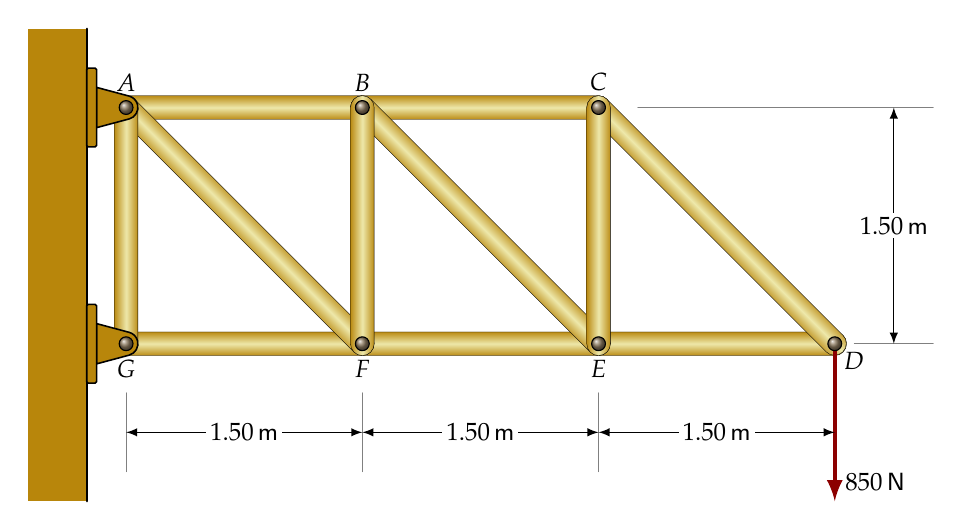
\begin{tikzpicture}[scale=\scale, line cap=round]

	\small

	\coordinate (A) at (0,3);
	\coordinate (B)	at (3,3);
	\coordinate (C) at (6,3);
	\coordinate (D) at (9,0);
	\coordinate (E) at (6,0);
	\coordinate (F) at (3,0);
	\coordinate (G) at (0,0);
	\coordinate (BCa) at ($(B)!.5!(C)+(0,0.5)$);
	\coordinate (EFa) at ($(E)!.5!(F)+(0,-0.5)$);

	\gettikzxy{(A)}{\ax}{\ay}
	\gettikzxy{(B)}{\bx}{\by}
	\gettikzxy{(C)}{\cx}{\cy}
	\gettikzxy{(D)}{\ddx}{\ddy}
	\gettikzxy{(E)}{\eex}{\eey}
	\gettikzxy{(F)}{\fx}{\fy}
	\gettikzxy{(G)}{\gx}{\gy}
	
	\Meme{A}{B}{DarkGoldenrod}{PaleGoldenrod}{black}{0.3}{0.15}{0.125}
	\Meme{C}{B}{DarkGoldenrod}{PaleGoldenrod}{black}{0.3}{0.15}{0.125}
	
	\Meme{E}{D}{DarkGoldenrod}{PaleGoldenrod}{black}{0.3}{0.15}{0.125}
	\Meme{E}{F}{DarkGoldenrod}{PaleGoldenrod}{black}{0.3}{0.15}{0.125}
	\Meme{G}{F}{DarkGoldenrod}{PaleGoldenrod}{black}{0.3}{0.15}{0.125}
	\Meme{C}{D}{DarkGoldenrod}{PaleGoldenrod}{black}{0.3}{0.15}{0.125}
	\Meme{B}{E}{DarkGoldenrod}{PaleGoldenrod}{black}{0.3}{0.15}{0.125}
	\Meme{A}{F}{DarkGoldenrod}{PaleGoldenrod}{black}{0.3}{0.15}{0.125}
	\Meme{A}{G}{DarkGoldenrod}{PaleGoldenrod}{black}{0.3}{0.15}{0.125}
	\Meme{B}{F}{DarkGoldenrod}{PaleGoldenrod}{black}{0.3}{0.15}{0.125}
	\Meme{C}{E}{DarkGoldenrod}{PaleGoldenrod}{black}{0.3}{0.15}{0.125}
	

	\draw[ultra thick, -latex, saitMaroon] (D)--+(0,-2)node[above right, black]{\small $ 850\,\textsf{N}$ };

	% \only<1-3>{
		\node[above, outer sep = 1mm] at (A) {\small $ A $};
	% }
	% \only<4->{
		% \node[above left, outer sep = 1mm] at (A) {\small $ A $};
		% \draw[very thick, saitRed, -latex] (A)--+(0:1.25)node[above, outer sep=0.5mm,xshift=0.5mm]{$ R_{Ax} $};
		% \draw[very thick, saitRed, -latex] (A)--+(90:1)node[below right, outer sep=0.5mm, yshift=0.75mm,xshift=-0.25mm]{$ R_{Ay} $};
		% \draw[very thick, saitRed, -latex] (G)--+(0:1.25)node[above, outer sep=0.75mm]{$ R_{Gx} $};
		% \draw[very thick, saitRed, -latex] (G)--+(90:1.25)node[right, outer sep=0.75mm]{$ R_{Gy} $};
	% }
	
	\node[above, outer sep = 1mm] at (B) {\small $ B $};
	\node[above, outer sep = 1mm] at (C) {\small $ C $};
	\node[below right] at (D) {\small $ D $};
	\node[below, outer sep = 1mm] at (E) {\small $ E $};
	\node[below, outer sep = 1mm] at (F) {\small $ F $};
	\node[below, outer sep = 1mm] at (G) {\small $ G $};

	% \only<1-3>{
		\fill[DarkGoldenrod]($(A)+(-0.5,1)$) rectangle ($(G)+(-1.25,-2)$);
		\draw[thick]($(A)+(-0.5,1)$) -- ($(G)+(-0.5,-2)$);
		\PC[-90]{A}{DarkGoldenrod}{black}{0.5}{0.2}
		\PC[-90]{G}{DarkGoldenrod}{black}{0.5}{0.2}
	% }
	% \only<4->{
	% 	\begin{scope}[opacity=0]
	% 		\fill[DarkGoldenrod,opacity=0]($(A)+(-0.5,1)$) rectangle ($(G)+(-1.25,-2)$);
	% 		\draw[thick,opacity=0]($(A)+(-0.5,1)$) -- ($(G)+(-0.5,-2)$);
	% 		\PC[-90]{A}{DarkGoldenrod}{black}{0.5}{0.2}
	% 		\PC[-90]{G}{DarkGoldenrod}{black}{0.5}{0.2}
	% 	\end{scope}		
	% }
	
	

	

	\draw[thin, gray]($ (E)+(0,-0.625)$)--+(0,-1);
	\draw[thin, gray]($ (F)+(0,-0.625)$)--+(0,-1);
	\draw[thin, gray]($ (G)+(0,-0.625)$)--+(0,-1);

	\draw[thin, gray]($ (D)+(0:0.25)$)--+(0:1);
	\draw[thin, gray]($ (C)+(0:0.5)$)--+(0:3.75);
	
	\draw[latex-latex] ($(D)+(0.75,0)$)--($(C)+(3.75,0)$)node[midway, fill=white, inner sep=0.5mm]{$ 1.50\,\textsf{m} $};

	\draw[latex-latex] ($(G)+(0,-1.125)$)--($(F)+(0,-1.125)$)node[midway, fill=white, inner sep=0.5mm]{$ 1.50\,\textsf{m} $};
	\draw[latex-latex] ($(E)+(0,-1.125)$)--($(F)+(0,-1.125)$)node[midway, fill=white, inner sep=0.5mm]{$ 1.50\,\textsf{m} $};
	\draw[latex-latex] ($(D)+(0,-1.125)$)--($(E)+(0,-1.125)$)node[midway, fill=white, inner sep=0.5mm]{$ 1.50\,\textsf{m} $};

	% \only<3>{
	% 	\begin{scope}[rotate around = {10:(\bx/2+\cx/2, \by/2+\eey/2)}]
	% 		\draw[ultra thick, LimeGreen] (\bx/2+\cx/2, \cy+0.5cm)--(\fx/2+\eex/2, \fy-0.5cm);
	% 		\node[above, LimeGreen!62.55!black] at (\bx/2+\cx/2, \cy+0.5cm) {$a$};
	% 		\node[below, LimeGreen!62.55!black] at (\fx/2+\eex/2, \fy-0.5cm) {$a$};
	% 	\end{scope}
	% }
	% \only<4->{
	% 	\begin{scope}[rotate around = {10:(\bx/2+\cx/2, \by/2+\eey/2)}]
	% 		\fill[white] (\bx+0.75cm, \by+0.75cm) rectangle (\eex-0.75cm, \eey-0.75cm);
	% 	\end{scope}
	% }
	% \only<5->{
	% 	\tikzset{outer sep=-0.25mm}
	% 	\draw[very thick, -latex] (B)--+(0:0.875)node[right,xshift=-0.5mm]{$F_{BC}$};
	% 	\draw[very thick, -latex] (C)--+(180:1.4);%node[below]{$F_{BC}$};
	% 	\draw[very thick, -latex] (F)--+(0:1.4)node[right,xshift=-0.5mm]{$F_{EF}$};
	% 	\draw[very thick, -latex] (E)--+(180:0.875);%node[below]{$F_{EF}$};
	% 	\draw[very thick, -latex] (B)--+(-45:1.5)node[below right,xshift=0.75mm, yshift=-1mm]{$F_{BE}$};
	% 	\draw[very thick, -latex] ($(E)+(135:0)$)--+(135:1.5);%node[above]{$F_{BE}$};
	% }

	% \path(-1.5,4) rectangle (10.5,-2);
	% \draw[red](-1.5,4) rectangle (10.5,-2);

	\foreach \coord in {A,B,C,D,...,G}{
		\filldraw[ball color = NavajoWhite4] (\coord) circle (2.5pt);
	};
	
\end{tikzpicture}

		\parb
		\cmini[0.75]{
			\centering
			Use the method of sections to determine the internal forces in members $BC$, $CH$ and $GH$.
		}			
		\pars
		\addtocounter{\tcbcounter}{-1}
	\end{myexam}
\end{frame}
	
%%%%%%%%%%%%%%%%%%%%%%%%%%%%%%%%%%%%%%%%%%%%%%%%%%%%%%%%%%%%%%%%%%%%%%%%%%%%%%%%%%%%%%%%%%%%%%%%%%%%

\begin{frame}	
	
	\begin{statsbox}[height=5.25cm, top=0mm]{}
		\def\scale{0.825}			
		\centering
		
%%%%%%%%%%%%%%%%%%%%%%% TRUSS %%%%%%%%%%%%%%%%%%%%%%%%%%%%%%%%%%%%%%%%%%%%%%%%%%%%%%%%%%%%%%%%%%%%%
\begin{tikzpicture}[scale=\scale, line cap=round]

	\footnotesize

	\coordinate (A) at (0,3);
	\coordinate (B)	at (3,3);
	\coordinate (C) at (6,3);
	\coordinate (D) at (9,0);
	\coordinate (E) at (6,0);
	\coordinate (F) at (3,0);
	\coordinate (G) at (0,0);
	\coordinate (BC) at ($(B)!.5!(C)$);
	\coordinate (EF) at ($(E)!.5!(F)$);
	\coordinate (BE) at ($(B)!.5!(E)$);

	\gettikzxy{(A)}{\ax}{\ay}
	\gettikzxy{(B)}{\bx}{\by}
	\gettikzxy{(C)}{\cx}{\cy}
	\gettikzxy{(D)}{\ddx}{\ddy}
	\gettikzxy{(E)}{\eex}{\eey}
	\gettikzxy{(F)}{\fx}{\fy}
	\gettikzxy{(G)}{\gx}{\gy}
	
	\only<1-9>{
		\Meme{A}{B}{DarkGoldenrod}{PaleGoldenrod}{black}{0.3}{0.15}{0.125}
		\Meme{C}{B}{DarkGoldenrod}{PaleGoldenrod}{black}{0.3}{0.15}{0.125}
		\Meme{E}{F}{DarkGoldenrod}{PaleGoldenrod}{black}{0.3}{0.15}{0.125}
		\Meme{G}{F}{DarkGoldenrod}{PaleGoldenrod}{black}{0.3}{0.15}{0.125}
		\Meme{B}{E}{DarkGoldenrod}{PaleGoldenrod}{black}{0.3}{0.15}{0.125}
		\Meme{A}{F}{DarkGoldenrod}{PaleGoldenrod}{black}{0.3}{0.15}{0.125}
		\Meme{A}{G}{DarkGoldenrod}{PaleGoldenrod}{black}{0.3}{0.15}{0.125}
		\Meme{B}{F}{DarkGoldenrod}{PaleGoldenrod}{black}{0.3}{0.15}{0.125}
	}
	\only<10->{		
		\Meme{A}{B}{Cornsilk3}{white}{gray!50}{0.3}{0.15}{0.125}
		\Meme{BC}{B}{Cornsilk3}{white}{gray!50}{0.3}{0.15}{0.125}
		\Meme{EF}{F}{Cornsilk3}{white}{gray!50}{0.3}{0.15}{0.125}
		\Meme{G}{F}{Cornsilk3}{white}{gray!50}{0.3}{0.15}{0.125}
		\Meme{B}{BE}{Cornsilk3}{white}{gray!50}{0.3}{0.15}{0.125}
		\Meme{A}{F}{Cornsilk3}{white}{gray!50}{0.3}{0.15}{0.125}
		\Meme{A}{G}{Cornsilk3}{white}{gray!50}{0.3}{0.15}{0.125}
		\Meme{A}{G}{Cornsilk3}{white}{gray!50}{0.3}{0.15}{0.125}
		\Meme{B}{F}{Cornsilk3}{white}{gray!50}{0.3}{0.15}{0.125}
		\Meme{E}{BE}{DarkGoldenrod}{PaleGoldenrod}{black}{0.3}{0.15}{0.125}		
		\Meme{E}{EF}{DarkGoldenrod}{PaleGoldenrod}{black}{0.3}{0.15}{0.125}		
		\Meme{C}{BC}{DarkGoldenrod}{PaleGoldenrod}{black}{0.3}{0.15}{0.125}		
	}
	\Meme{E}{D}{DarkGoldenrod}{PaleGoldenrod}{black}{0.3}{0.15}{0.125}	
	\Meme{C}{D}{DarkGoldenrod}{PaleGoldenrod}{black}{0.3}{0.15}{0.125}	
	\Meme{C}{E}{DarkGoldenrod}{PaleGoldenrod}{black}{0.3}{0.15}{0.125}
	

	\draw[very thick, -latex, saitMaroon] (D)--+(0,-1.5)node[above right, black,
	yshift=-0.75mm]{ $ 850\,\textsf{N}$ };

	\only<1-7, 10->{
		\node[above, outer sep = 1mm] at (A) { $ A $};
	}
	\only<8-9>{
		\node[above left, outer sep = 0.5mm] at (A) { $ A $};
	}
	\only<8-9>{			
		\draw[very thick, saitRed, -latex] (A)--+(0:1.25)node[above, outer sep=1mm,xshift=2mm]{\small $ R_{Ax} $};
		\draw[very thick, saitRed, -latex] (A)--+(90:1)node[below right, outer sep=0.5mm, yshift=0.75mm,xshift=-0.25mm]{\small $ R_{Ay} $};
		\draw[very thick, saitRed, -latex] (G)--+(0:1.25)node[above, outer sep=1mm]{\small $ R_{Gx} $};
		\draw[very thick, saitRed, -latex] (G)--+(90:1.25)node[right, outer sep=1mm]{\small $ R_{Gy} $};
	}
	
	\node[above, outer sep = 1.25mm] at (B) { $ B $};
	\node[above, outer sep = 1.25mm] at (C) { $ C $};
	\node[below right, outer sep = 0.5mm] at (D) { $ D $};
	\node[below, outer sep = 1.25mm] at (E) { $ E $};
	\node[below, outer sep = 1.25mm] at (F) { $ F $};
	\node[below, outer sep = 1.25mm] at (G) { $ G $};

	\draw[thin, gray]($ (E)+(0,-0.625)$)--+(0,-0.5);
	\draw[thin, gray]($ (F)+(0,-0.625)$)--+(0,-0.5);
	\draw[thin, gray]($ (G)+(0,-0.625)$)--+(0,-0.5);
	\draw[thin, gray]($ (D)+(0:0.25)$)--+(0:1);
	\draw[thin, gray]($ (C)+(0:0.5)$)--+(0:3.75);	
	
	\draw[latex-latex] ($(D)+(0.75,0)$)--($(C)+(3.75,0)$)node[midway, fill=white, inner sep=0.5mm]{$ 1.50\,\textsf{m} $};
	\draw[latex-latex] ($(G)+(0,-0.875)$)--($(F)+(0,-0.875)$)node[midway, fill=white, inner sep=0.5mm]{$ 1.50\,\textsf{m} $};
	\draw[latex-latex] ($(E)+(0,-0.875)$)--($(F)+(0,-0.875)$)node[midway, fill=white, inner sep=0.5mm]{$ 1.50\,\textsf{m} $};
	\draw[latex-latex] ($(D)+(0,-0.875)$)--($(E)+(0,-0.875)$)node[midway, fill=white, inner sep=0.5mm]{$ 1.50\,\textsf{m} $};

	\only<2>{
		\begin{scope}[rotate around = {10:(\bx/2+\cx/2, \by/2+\eey/2)}]
			\draw[ultra thick, LimeGreen] (\bx/2+\cx/2, \cy+0.5cm)--(\fx/2+\eex/2, \fy-0.5cm);
			\node[above, LimeGreen!62.55!black] at (\bx/2+\cx/2+0.187cm, \cy+0.25cm) {$a$};
			\node[below, LimeGreen!62.55!black] at (\fx/2+\eex/2 +0.25cm, \fy-0.25cm) {$a$};
		\end{scope}
	}
	\only<3->{
		\begin{scope}[rotate around = {10:(\bx/2+\cx/2, \by/2+\eey/2)}]
			\fill[white] (\bx+0.75cm, \by+0.5cm) rectangle (\eex-0.75cm, \eey-0.5cm);
		\end{scope}
	}

	\only<1-2>{
		\fill[DarkGoldenrod]($(A)+(-0.5,1)$) rectangle ($(G)+(-1.25,-1.5)$);
		\draw[thick]($(A)+(-0.5,1)$) -- ($(G)+(-0.5,-1.5)$);
		\PC[-90]{A}{DarkGoldenrod}{black}{0.5}{0.2}
		\PC[-90]{G}{DarkGoldenrod}{black}{0.5}{0.2}
	}

	\only<3->{
		\begin{scope}[opacity=0]
			\fill[DarkGoldenrod,opacity=0]($(A)+(-0.5,1)$) rectangle ($(G)+(-1.25,-2)$);
			\draw[thick,opacity=0]($(A)+(-0.5,1)$) -- ($(G)+(-0.5,-2)$);
			\PC[-90]{A}{DarkGoldenrod}{black}{0.5}{0.2}
			\PC[-90]{G}{DarkGoldenrod}{black}{0.5}{0.2}
		\end{scope}		
	}
	\only<4->{
		\tikzset{outer sep=-0.25mm}		
		\draw[very thick, -latex] (C)--+(180:1.4)node[left]{$F_{BC}$};		
		\draw[very thick, -latex] (E)--+(180:1.0625)node[left,xshift=0.125mm]{$F_{EF}$};		
		\draw[very thick, -latex] ($(E)+(135:0)$)--+(135:1.5)node[xshift=-3mm, yshift=3.5mm]{$F_{BE}$};
	}	
	\only<4-9>{
		\tikzset{outer sep=-0.25mm}
		\draw[very thick, -latex] (B)--+(0:1);
		\draw[very thick, -latex] (B)--+(-45:1.5);
		\draw[very thick, -latex] (F)--+(0:1.4);
	}

	\foreach \coord in {A,B,C,D,...,G}{
		\filldraw[ball color = NavajoWhite4] (\coord) circle (2.5pt);
	};
	\only<10->{
		\foreach \coord in {A,B,F,G}{
			\fill[thin, ball color = Cornsilk2] (\coord) circle (2.5pt);
		};
	}

	\pgfresetboundingbox
	\path(-1.5,4.25) rectangle (10.75,-1.75);
	% \draw[red](-1.5,4.25) rectangle (10.75,-1.75);
	
\end{tikzpicture}
			
	\end{statsbox}
	\parm
	\only<1-7>{
		\begin{statsbox}[height=2.5cm]{The Method of Sections}
			\only<1-4>{
				\begin{itemize}
					\item<1-> The method of sections technique is widely used in engineering. 
					\item<2-> It involves drawing a section $a\!-\!a$ through a structure or member.
					\item<3-> Then the segments on each side of the section are also be in equilibrium.
					\item<4-> The section 'exposes' the internal forces in cut members.				
				\end{itemize}
			}
			\only<5-7>{
				\begin{itemize}				
					\item <5-> We are free to place our section wherever is most convenient.\parm
					\item <6-> We generally look for a section that 'cuts' the members we need. \parm
					\item <7->	Then we choose whichever is the easier of the two segments to analyze.
				\end{itemize}
			}
		\end{statsbox}
	}
		\only<8-9>{
			\begin{myexam}[height=2.5cm, left=0mm]{Solution}{}
				\only<8-9>{
					\begin{itemize}
						\item<8-> The right segment is the easiest to analyze since it only contains a single external force.					
						\item<9-> Note that in this case we only have the one choice since the reactions at $A$ and $G$ are '{\bf statically indeterminate}.' (That is, we can't determine them using only the equilibrium equations. Why is this?) 
						\item <10-> ten			
					\end{itemize}
				}
			\end{myexam}
		}
		\only<10->{
			\begin{myexam}[height=2.5cm, left=0mm]{Solution}{}
				\small
				\only<10>{
					\begin{align*}
						\Sigma M_E &= F_{BC}\cd(1.50\,\textsf{m}) - (850\,\textsf{N})\cd (1.50\,\textsf{m}) = 0\\\\
						\Ra F_{BC} &= 850\,\textsf{N}
					\end{align*}
				}
				\only<11>{
					\begin{align*}
						\Sigma M_B &= -F_{EF}\cd(1.50\,\textsf{m}) - (850\,\textsf{N})\cd (3.00\,\textsf{m}) = 0\\\\
						\Ra F_{EF} &= -1700\,\textsf{N}
					\end{align*}
				}
				\only<12-13>{
					\begin{align*}
						\Sigma F_y &= -F_{BE}\cd\sin 45\deg - 850\,\textsf{N} = 0\\\\
						\Ra F_{BE} &= -1202.1\,\textsf{N}
					\end{align*}
				}
			\end{myexam}
		}
		\only<13->{
			\begin{textblock*}{\columnwidth}(0.875cm,0.125cm)
				\def\modalFill{\bgcolor}
				\tikz{%color
  \fill[fill=\modalFill, opacity=0.875] (0.1,0.3) rectangle (12.7,9.45);
}	
			\end{textblock*}
				
			\only<13->{
				\begin{textblock*}{5cm}(7cm,0.5cm)
					\begin{statsbox}{The Answers}
						\small
						\begin{align*}
							BC &= 850\,\textsf{N}\quad\textsf{(Tension)}\\[0.25em]
							BE &= 1200\,\textsf{N}\quad\textsf{(Compression)}\\[0.25em]
							EF &= 1700\,\textsf{N}\quad\textsf{(Compression)}
						\end{align*}
						\par
					\end{statsbox}
				\end{textblock*}
			}
			
			\only<14->{
				\begin{textblock*}{9cm}(3cm,3cm)
					\begin{statsbox}[left = 0mm, right=2mm]{Note:}
						\small
						\begin{enumerate}
							\item<14-> If any structure (not only a truss) is in equilibrium, then any section will cut it into two segments, each of which is itself in equilibrium. 
							\item<15-> To solve for more than three truss members, it is necessary to repeat the method of sections using a different section (one that cuts the additional members required by the problem).
							\item<16-> We can use all three equilibrium equations $\Sigma M = 0$, $\Sigma F_x=0$ and $\Sigma F_y=0$ but it is often less work to take moments about conveniently located joints.
							\item<17> It is not necessary to take moments using joints in the 'active' segment. Moments can be taken about anywhere on the truss -- or even anywhere on the plane in which the truss is situated. If a structure is in equilibrium, its moments about any point in the plane still sum to zero.
						\end{enumerate}
					\end{statsbox}
				\end{textblock*}
			}	
		}
		% \addtocounter{framenumber}{0}
\end{frame}
%%%%%%%%%%%%%%%%%%%%%%%%%%%%%%%%%%%%%%%%%%%%%%%%%%%%%%%%%%%%%%%%%%%%%%%%%%%%%%%%%%%%%%%%%%%%%%%%%%%%
\begin{frame}{}
	\def\scale{0.5}
	\begin{myexam}{}{}
		\parb\centering
		
%%%%%%%%%%%%%%%%%%%%%%% TRUSS %%%%%%%%%%%%%%%%%%%%%%%%%%%%%%%%%%%%%%%%%%%%%%%%%%%%%%%%%%%%%%%%%%%%%
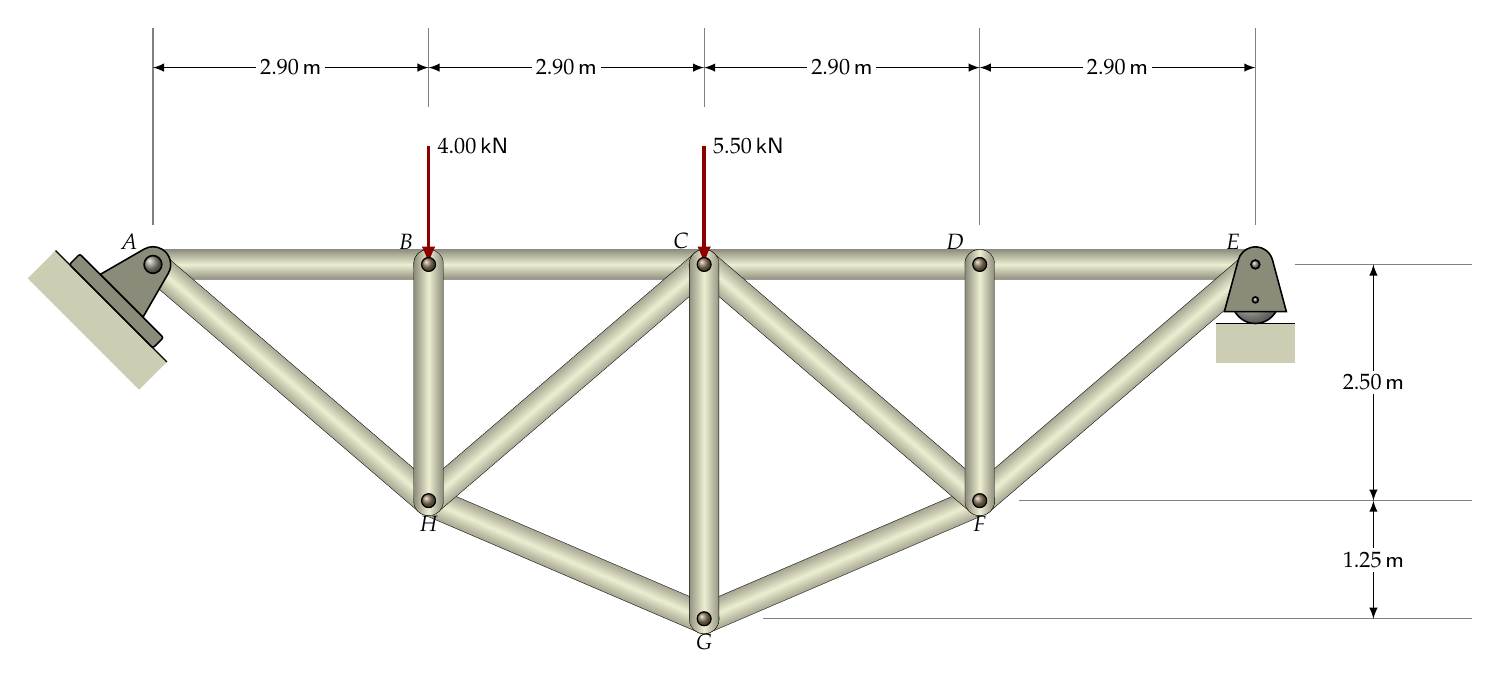
\begin{tikzpicture}[scale=\scale]

	\footnotesize

	\coordinate (A) at (0,0);
	\coordinate (B)	at (3.5,0);
	\coordinate (C) at (7,0);
	\coordinate (D) at (10.5,0);
	\coordinate (E) at (14,0);
	\coordinate (F) at (10.5,-3);
	\coordinate (G) at (7,-4.5);
	\coordinate (H) at (3.5,-3);	

	\gettikzxy{(A)}{\ax}{\ay}
	\gettikzxy{(B)}{\bx}{\by}
	\gettikzxy{(C)}{\cx}{\cy}
	\gettikzxy{(D)}{\ddx}{\ddy}
	\gettikzxy{(E)}{\eex}{\eey}
	\gettikzxy{(F)}{\fx}{\fy}
	\gettikzxy{(G)}{\gx}{\gy}
	
	\Meme{A}{B}{LightYellow4}{LightYellow2}{black}{0.375}{0.175}{0.125}
	\Meme{C}{B}{LightYellow4}{LightYellow2}{black}{0.375}{0.175}{0.125}
	\Meme{C}{D}{LightYellow4}{LightYellow2}{black}{0.375}{0.175}{0.125}
	\Meme{E}{D}{LightYellow4}{LightYellow2}{black}{0.375}{0.175}{0.125}
	\Meme{E}{F}{LightYellow4}{LightYellow2}{black}{0.375}{0.175}{0.125}
	\Meme{G}{F}{LightYellow4}{LightYellow2}{black}{0.375}{0.175}{0.125}
	\Meme{G}{H}{LightYellow4}{LightYellow2}{black}{0.375}{0.175}{0.125}
	\Meme{A}{H}{LightYellow4}{LightYellow2}{black}{0.375}{0.175}{0.125}
	\Meme{C}{H}{LightYellow4}{LightYellow2}{black}{0.375}{0.175}{0.125}
	\Meme{C}{F}{LightYellow4}{LightYellow2}{black}{0.375}{0.175}{0.125}
	\Meme{B}{H}{LightYellow4}{LightYellow2}{black}{0.375}{0.175}{0.125}
	\Meme{C}{G}{LightYellow4}{LightYellow2}{black}{0.375}{0.175}{0.125}
	\Meme{D}{F}{LightYellow4}{LightYellow2}{black}{0.375}{0.175}{0.125}

	\draw[very thick, latex-, saitMaroon] (B)--+(0,1.5)node[right, black]{$ 4.00\,\textsf{kN}$ };
	\draw[very thick, latex-, saitMaroon] (C)--+(0,1.5)node[right, black]{$ 5.50\,\textsf{kN}$ };

	\node[above left, outer sep = 1mm] at (A) {$ A $};
	\node[above left, outer sep = 1mm] at (B) {$ B $};
	\node[above left, outer sep = 1mm] at (C) {$ C $};
	\node[above left, outer sep = 1mm] at (D) {$ D $};
	\node[above left, outer sep = 1mm] at (E) {$ E $};
	\node[below, outer sep = 1mm] at (F) {$ F $};
	\node[below, outer sep = 1mm] at (G) {$ G $};
	\node[below, outer sep = 1mm] at (H) {$ H $};
	

	\foreach \coord in {A,B,C,D,...,H}{
		\filldraw[ball color = NavajoWhite4] (\coord) circle (2.5pt);
	};

	\begin{scope}[rotate around= {315:(A)}]
		\fill[LightYellow3] ($(A)+(-1,-0.75)$) rectangle ($(A)+(1,-1.25)$);
		\draw  ($(A)+(-1,-0.75)$) -- ($(A)+(1.,-0.75)$);
		\PC{A}{LightYellow4}{black}{0.75}{0.2}
	\end{scope}
	\fill[LightYellow3] ($(E)+(-0.5,-0.75)$) rectangle ($(E)+(0.5,-1.25)$);
	\draw  ($(E)+(-0.5,-0.75)$) -- ($(E)+(0.5,-0.75)$);
	\Rone{E}{LightYellow4}{black}{0.75}{0.2}	

	\draw[thin, gray]($ (E)+(0.5,0)$)--+(2.25,0);
	\draw[thin, gray]($ (F)+(0.5,0)$)--+(5.75,0);
	\draw[thin, gray]($ (G)+(0.75,0)$)--+(9,0);

	\draw[thin, gray]($ (A)+(90:0.5)$)--+(90:2.5);
	\draw[thin, gray]($ (D)+(90:0.5)$)--+(90:2.5);
	\draw[thin, gray]($ (E)+(90:0.5)$)--+(90:2.5);
	\draw[thin, gray]($ (B)+(90:2)$)--+(90:1);
	\draw[thin, gray]($ (C)+(90:2)$)--+(90:1);
	
	\draw[latex-latex] ($(E)+(1.5,0)$)--($(F)+(5,0)$)node[midway, fill=white, inner sep=0.5mm]{$ 2.50\,\textsf{m} $};
	\draw[latex-latex] ($(G)+(8.5,0)$)--($(F)+(5,0)$)node[midway, fill=white, inner sep=0.5mm]{$ 1.25\,\textsf{m} $};

	\draw[latex-latex] ($(A)+(0,2.5)$)--($(B)+(0,2.5)$)node[midway, fill=white, inner sep=0.5mm]{$ 2.90\,\textsf{m} $};
	\draw[latex-latex] ($(C)+(0,2.5)$)--($(B)+(0,2.5)$)node[midway, fill=white, inner sep=0.5mm]{$ 2.90\,\textsf{m} $};
	\draw[latex-latex] ($(C)+(0,2.5)$)--($(D)+(0,2.5)$)node[midway, fill=white, inner sep=0.5mm]{$ 2.90\,\textsf{m} $};
	\draw[latex-latex] ($(E)+(0,2.5)$)--($(D)+(0,2.5)$)node[midway, fill=white, inner sep=0.5mm]{$ 2.90\,\textsf{m} $};
	
	
\end{tikzpicture}

		\pars
		Use the method of sections to determine the internal forces in members $BC$, $CH$ and $GH$.
		\pars
	\end{myexam}
\end{frame}

%%%%%%%%%%%%%%%%%%%%%%%%%%%%%%%%%%%%%%%%%%%%%%%%%%%%%%%%%%%%%%%%%%%%%%%%%%%%%%%%%%%%%%%%%%%%%%%%%%%%
\begin{frame}{}
	\def\scale{0.5125}
	\begin{myexam}{}{}
		\parb\centering
		\input{../../pikz/08MoS/08MoS06.tex}
		\pars
		Use the method of sections to determine the internal forces in members $BC$, $CH$ and $GH$.
		\pars
	\end{myexam}
\end{frame}

%%%%%%%%%%%%%%%%%%%%%%%%%%%%%%%%%%%%%%%%%%%%%%%%%%%%%%%%%%%%%%%%%%%%%%%%%%%%%%%%%%%%%%%%%%%%%%%%%%%%
\begin{frame}{}
	\def\scale{0.5125}
	\begin{myexer}{}{}
		\parb\centering
		\input{../../pikz/08MoS/08MoS07.tex}
		\pars
		An alternative design is being considered for the previous example. 
		Use the method of sections to determine the internal forces in members $BC$, $BG$ and $GH$. How do they compare to the previous results?
		\pars
	\end{myexer}
\end{frame}


%%%%%%%%%%%%%%%%%%%%%%%%%%%%%%%%%%%%%%%%%%%%%%%%%%%%%%%%%%%%%%%%%%%%%%%%%%%%%%%%%%%%%%%%%%%%%%%%%%%%

\begin{frame}{}
	\def\scale{0.45}
	\begin{myexam}{}{}
		\parb\centering
		
%%%%%%%%%%%%%%%%%%%%%%% TRUSS %%%%%%%%%%%%%%%%%%%%%%%%%%%%%%%%%%%%%%%%%%%%%%%%%%%%%%%%%%%%%%%%%%%%%
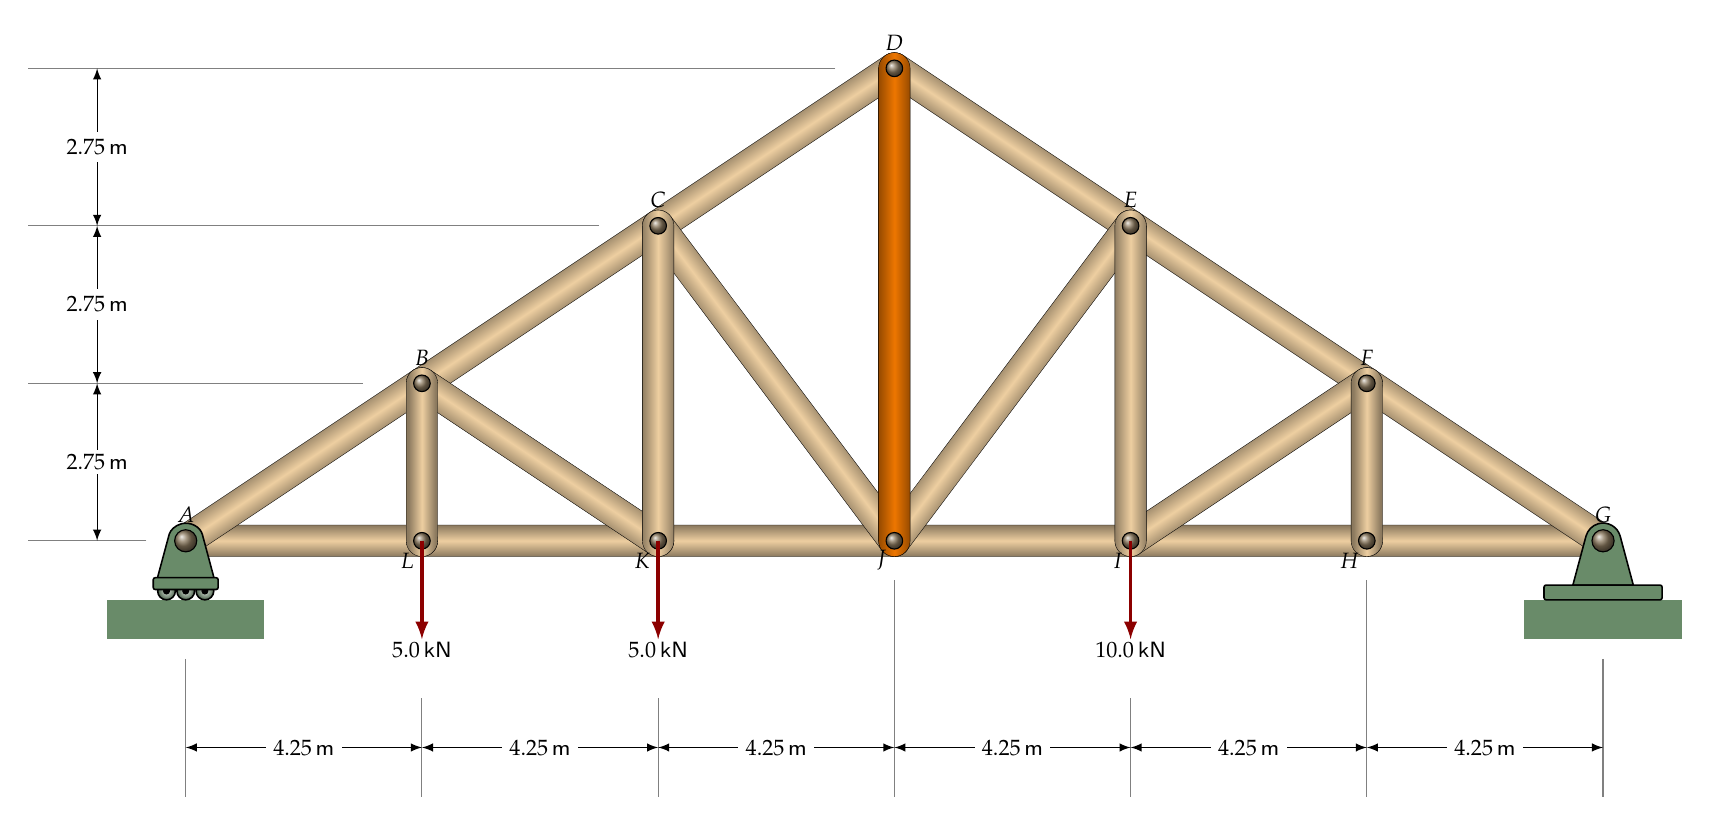
\begin{tikzpicture}[scale=\scale]

	\footnotesize

	\coordinate (A) at (0,0);
	\coordinate (B)	at (3,2);
	\coordinate (C) at (6,4);
	\coordinate (D) at (9,6);
	\coordinate (E) at (12,4);
	\coordinate (F) at (15,2);
	\coordinate (G) at (18,0);
	\coordinate (H) at (15,0);
	\coordinate (I) at (12,0);
	\coordinate (J) at (9,0);
	\coordinate (K) at (6,0);
	\coordinate (L) at (3,0);
	

	\gettikzxy{(A)}{\ax}{\ay}
	\gettikzxy{(B)}{\bx}{\by}
	\gettikzxy{(C)}{\cx}{\cy}
	\gettikzxy{(D)}{\ddx}{\ddy}
	\gettikzxy{(E)}{\eex}{\eey}
	\gettikzxy{(F)}{\fx}{\fy}
	\gettikzxy{(G)}{\gx}{\gy}
	

	
	\Meme{C}{B}{NavajoWhite4}{NavajoWhite2}{black}{0.4}{0.2}{0.125}
	\Meme{C}{D}{NavajoWhite4}{NavajoWhite2}{black}{0.4}{0.2}{0.125}
	\Meme{E}{D}{NavajoWhite4}{NavajoWhite2}{black}{0.4}{0.2}{0.125}
	\Meme{E}{F}{NavajoWhite4}{NavajoWhite2}{black}{0.4}{0.2}{0.125}
	
	\Meme{G}{H}{NavajoWhite4}{NavajoWhite2}{black}{0.4}{0.2}{0.125}
	\Meme{I}{H}{NavajoWhite4}{NavajoWhite2}{black}{0.4}{0.2}{0.125}
	\Meme{I}{J}{NavajoWhite4}{NavajoWhite2}{black}{0.4}{0.2}{0.125}
	\Meme{K}{J}{NavajoWhite4}{NavajoWhite2}{black}{0.4}{0.2}{0.125}
	\Meme{K}{L}{NavajoWhite4}{NavajoWhite2}{black}{0.4}{0.2}{0.125}
	\Meme{A}{L}{NavajoWhite4}{NavajoWhite2}{black}{0.4}{0.2}{0.125}
	\Meme{A}{B}{NavajoWhite4}{NavajoWhite2}{black}{0.4}{0.2}{0.125}
	\Meme{G}{F}{NavajoWhite4}{NavajoWhite2}{black}{0.4}{0.2}{0.125}
	\Meme{B}{K}{NavajoWhite4}{NavajoWhite2}{black}{0.4}{0.2}{0.125}
	\Meme{C}{J}{NavajoWhite4}{NavajoWhite2}{black}{0.4}{0.2}{0.125}
	\Meme{E}{J}{NavajoWhite4}{NavajoWhite2}{black}{0.4}{0.2}{0.125}
	\Meme{F}{I}{NavajoWhite4}{NavajoWhite2}{black}{0.4}{0.2}{0.125}
	\Meme{B}{L}{NavajoWhite4}{NavajoWhite2}{black}{0.4}{0.2}{0.125}
	\Meme{C}{K}{NavajoWhite4}{NavajoWhite2}{black}{0.4}{0.2}{0.125}
	\Meme{D}{J}{DarkOrange4}{DarkOrange2}{black}{0.4}{0.2}{0.125}
	\Meme{E}{I}{NavajoWhite4}{NavajoWhite2}{black}{0.4}{0.2}{0.125}
	\Meme{F}{H}{NavajoWhite4}{NavajoWhite2}{black}{0.4}{0.2}{0.125}

	
	

	\foreach \coord in {A,B,...,G}{
		\filldraw[ball color = NavajoWhite4] (\coord) circle (3pt)node[yshift=0.325cm] {$ \coord $};
	};
	\foreach \coord in {H, I, J, K, L}{
		\filldraw[ball color = NavajoWhite4] (\coord) circle (3pt)node[left, yshift=-0.25cm] {$ \coord $};		
	};	

	\fill[DarkSeaGreen4] ($(A)+(-1,-0.75)$) rectangle +(2,-0.5);
	\fill[DarkSeaGreen4] ($(G)+(-1,-0.75)$) rectangle +(2,-0.5);
	\PC{G}{DarkSeaGreen4}{black}{0.75}{0.2}
	\Roller{A}{DarkSeaGreen4}{black}{0.75}{0.2}
	\filldraw[ball color = NavajoWhite4] (A) circle (4pt);
	\filldraw[ball color = NavajoWhite4] (G) circle (4pt);

	\draw[thin, gray]($ (A)+(0,-1.5)$)--+(0,-1.75);
	\draw[thin, gray]($ (G)+(0,-1.5)$)--+(0,-1.75);
	\draw[thin, gray]($ (J)+(0,-.5)$)--+(0,-2.75);
	\draw[thin, gray]($ (H)+(0,-.5)$)--+(0,-2.75);
	\draw[thin, gray]($ (L)+(0,-2)$)--+(0,-1.25);
	\draw[thin, gray]($ (K)+(0,-2)$)--+(0,-1.25);
	\draw[thin, gray]($ (I)+(0,-2)$)--+(0,-1.25);
	\draw[thin, gray]($ (A)+(-0.5,0)$)--(-2, \ay);
	\draw[thin, gray]($ (B)+(-0.75,0)$)--(-2, \by);
	\draw[thin, gray]($ (C)+(-0.75,0)$)--(-2, \cy);
	\draw[thin, gray]($ (D)+(-0.75,0)$)--(-2, \ddy);

	\foreach \x in {0,1,2,...,5} {
		\draw[latex-latex] (\x*3, -2.625)--+(3,0)node[midway, fill=white]{$ 4.25\,\textsf{m} $};
	}
	\draw[latex-latex] (\ax-1.125cm, \ay)--(\ax-1.125cm, \by)node[midway, fill=white, inner sep = 0.5mm]{$ 2.75\,\textsf{m} $};
	\draw[latex-latex] (\ax-1.125cm, \by)--(\ax-1.125cm, \cy)node[midway, fill=white]{$ 2.75\,\textsf{m} $};
	\draw[latex-latex] (\ax-1.125cm, \cy)--(\ax-1.125cm, \ddy)node[midway, fill=white]{$ 2.75\,\textsf{m} $};
	
	
	% \foreach \coord in {F, G, ...,I }{
	% 	\filldraw[ball color = NavajoWhite4] (\coord) circle (2pt)node[above,outer sep = 0.125cm, xshift=-0.2cm] {$ \coord $};
	% 	\draw[thin, gray] ($(\coord)+(0,0.5)$)--+(0,1.5);
	% };
	% \draw[thin, gray] ($(E)+(0,0.5)$)--+(0,3.5);

	% \draw[thin, gray] ($(A)+(-0.75,0)$)--(\elx, \ay);
	% \draw[thin, gray] (\bx-0.75cm, \by)--(\elx, \by);
	% \draw[thin, gray] (\cx-0.75cm, \cy)--(\elx, \cy);
	% \draw[thin, gray] (\eex-0.5cm, \eey)--(\elx, \eey);
	% \draw[thin, gray] (\fx-0.75cm, \fy)--(\elx, \fy);



	\draw[very thick, -latex, statsMaroon] (L)--+(0,-1.25)node[below, black, yshift=0.75mm]{$ 5.0\,\textsf{kN}$ };
	\draw[very thick, -latex, statsMaroon] (K)--+(0,-1.25)node[below, black, yshift=0.75mm]{$ 5.0\,\textsf{kN}$ };
	\draw[very thick, -latex, statsMaroon] (I)--+(0,-1.25)node[below, black, yshift=0.75mm]{$ 10.0\,\textsf{kN}$ };

	% \draw[latex-latex] (\eex, 8)--(\fx,8)node[midway, fill=white] {$ 2.25\,\textsf{m} $};
	% \draw[latex-latex] (\fx, 8)--(\gx,8)node[midway, fill=white] {$ 2.25\,\textsf{m} $};
	% \draw[latex-latex] (\gx, 8)--(\hx,8)node[midway, fill=white] {$ 2.25\,\textsf{m} $};
	% \draw[latex-latex] (\hx, 8)--(\ix,8)node[midway, fill=white] {$ 2.25\,\textsf{m} $};

	% \draw[latex-latex] (\elx+0.75cm, \fy)--(\elx+0.75cm, \eey)node[midway, fill=white] {$ 1.50\,\textsf{m} $};
	% \draw[latex-latex] (\elx+0.75cm, \eey)--(\elx+0.75cm, \cy)node[midway, fill=white] {$ 1.50\,\textsf{m} $};
	% \draw[latex-latex] (\elx+0.75cm, \cy)--(\elx+0.75cm, \by)node[midway, fill=white] {$ 1.50\,\textsf{m} $};
	% \draw[latex-latex] (\elx+0.75cm, \by)--(\elx+0.75cm, \ay)node[midway, fill=white] {$ 1.50\,\textsf{m} $};
	
\end{tikzpicture}

		\parb
		Determine the internal force in $DJ$.
		\pars
	\end{myexam}
\end{frame}

%%%%%%%%%%%%%%%%%%%%%%%%%%%%%%%%%%%%%%%%%%%%%%%%%%%%%%%%%%%%%%%%%%%%%%%%%%%%%%%%%%%%%%%%%%%%%%%%%%%%
\begin{frame}{}
	\def\scale{0.575}
	
	\begin{myexam}{}{}
		\vspace{-1em}
		\mini[0.5]{
			\parb\centering
			
%%%%%%%%%%%%%%%%%%%%%%% TRUSS %%%%%%%%%%%%%%%%%%%%%%%%%%%%%%%%%%%%%%%%%%%%%%%%%%%%%%%%%%%%%%%%%%%%%
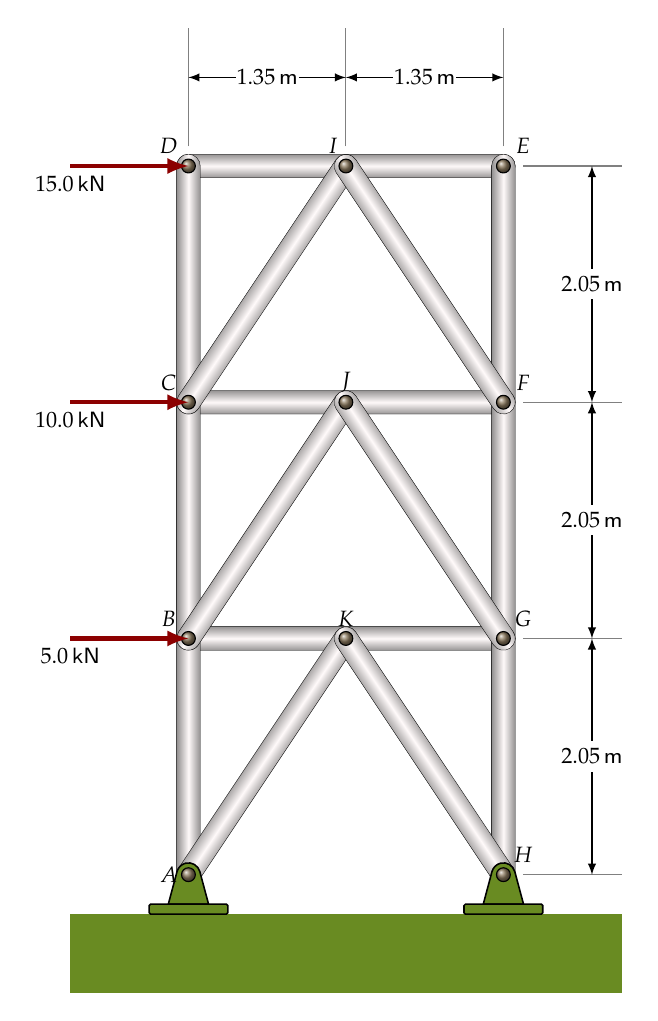
\begin{tikzpicture}[scale=\scale]

	\footnotesize

	\coordinate (A) at (0,0);
	\coordinate (B)	at (0,3);
	\coordinate (C) at (0,6);
	\coordinate (D) at (0,9);
	\coordinate (E) at (4,9);
	\coordinate (F) at (4,6);
	\coordinate (G) at (4,3);
	\coordinate (H) at (4,0);
	\coordinate (I) at (2,9);
	\coordinate (J) at (2,6);
	\coordinate (K) at (2,3);	

	\gettikzxy{(A)}{\ax}{\ay}
	\gettikzxy{(B)}{\bx}{\by}
	\gettikzxy{(C)}{\cx}{\cy}
	\gettikzxy{(D)}{\ddx}{\ddy}
	\gettikzxy{(E)}{\eex}{\eey}
	\gettikzxy{(F)}{\fx}{\fy}
	\gettikzxy{(G)}{\gx}{\gy}
	
	\Meme{B}{G}{Snow4}{Snow1}{black}{0.3}{0.15}{0.125}
	\Meme{C}{F}{Snow4}{Snow1}{black}{0.3}{0.15}{0.125}
	\Meme{E}{D}{Snow4}{Snow1}{black}{0.3}{0.15}{0.125}
	% \Meme{A}{H}{Snow4}{Snow1}{black}{0.3}{0.15}{0.125}
	\Meme{A}{B}{Snow4}{Snow1}{black}{0.3}{0.15}{0.125}
	\Meme{C}{B}{Snow4}{Snow1}{black}{0.3}{0.15}{0.125}
	\Meme{C}{D}{Snow4}{Snow1}{black}{0.3}{0.15}{0.125}
	
	\Meme{E}{F}{Snow4}{Snow1}{black}{0.3}{0.15}{0.125}
	\Meme{G}{F}{Snow4}{Snow1}{black}{0.3}{0.15}{0.125}
	\Meme{G}{H}{Snow4}{Snow1}{black}{0.3}{0.15}{0.125}
	
	\Meme{C}{I}{Snow4}{Snow1}{black}{0.3}{0.15}{0.125}
	\Meme{F}{I}{Snow4}{Snow1}{black}{0.3}{0.15}{0.125}
	\Meme{B}{J}{Snow4}{Snow1}{black}{0.3}{0.15}{0.125}
	\Meme{G}{J}{Snow4}{Snow1}{black}{0.3}{0.15}{0.125}
	\Meme{A}{K}{Snow4}{Snow1}{black}{0.3}{0.15}{0.125}
	\Meme{H}{K}{Snow4}{Snow1}{black}{0.3}{0.15}{0.125}

	\fill[OliveDrab4] ($(A)+(-1.5,-0.5)$)rectangle($(H)+(1.5,-1.5)$);
	\PC{A}{OliveDrab4}{black}{0.5}{0.2}
	\PC{H}{OliveDrab4}{black}{0.5}{0.2}	

	\foreach \coord in {B,C,D}{
		\filldraw[ball color = NavajoWhite4] (\coord) circle (2.5pt)node[xshift=-0.25cm,yshift=0.25cm] {$ \coord $};
	};
	\filldraw[ball color = NavajoWhite4] (A) circle (2.5pt)node[xshift=-0.25cm] {$ A $};
	\foreach \coord in {E,F,G,H}{
		\filldraw[ball color = NavajoWhite4] (\coord) circle (2.5pt)node[xshift=0.25cm,yshift=0.25cm] {$ \coord $};		
	};	
	\foreach \coord in {J,K}{
		\filldraw[ball color = NavajoWhite4] (\coord) circle (2.5pt)node[yshift=0.25cm] {$ \coord $};		
	};
	\filldraw[ball color = NavajoWhite4] (I) circle (2.5pt)node[left,yshift=0.25cm] {$ I $};		


	\draw[thin, gray]($ (E)+(0.25,0)$)--+(1.25,0);
	\draw[thin, gray]($ (F)+(0.25,0)$)--+(1.25,0);
	\draw[thin, gray]($ (G)+(0.25,0)$)--+(1.25,0);
	\draw[thin, gray]($ (H)+(0.25,0)$)--+(1.25,0);

	\draw[thin, gray]($ (D)+(0,0.25)$)--+(0,1.5);
	\draw[thin, gray]($ (I)+(0,0.25)$)--+(0,1.5);
	\draw[thin, gray]($ (E)+(0,0.25)$)--+(0,1.5);
	


	\draw[latex-latex] ($(H)+(1.125,0)$)--($(G)+(1.125,0)$)node[midway, fill=white]{$ 2.05\,\textsf{m} $};
	\draw[latex-latex] ($(G)+(1.125,0)$)--($(F)+(1.125,0)$)node[midway, fill=white]{$ 2.05\,\textsf{m} $};
	\draw[latex-latex] ($(E)+(1.125,0)$)--($(F)+(1.125,0)$)node[midway, fill=white]{$ 2.05\,\textsf{m} $};	
	\draw[latex-latex] ($(E)+(0,1.125)$)--($(I)+(0,1.125)$)node[midway, fill=white, inner sep = 0.1mm]{$ 1.35\,\textsf{m} $};	
	\draw[latex-latex] ($(D)+(0,1.125)$)--($(I)+(0,1.125)$)node[midway, fill=white, inner sep = 0.1mm]{$ 1.35\,\textsf{m} $};	
	
	\draw[ultra thick, latex-, saitMaroon] (B)--+(-1.5,0)node[below, black]{$ 5.0\,\textsf{kN}$ };
	\draw[ultra thick, latex-, saitMaroon] (C)--+(-1.5,0)node[below, black]{$ 10.0\,\textsf{kN}$ };
	\draw[ultra thick, latex-, saitMaroon] (D)--+(-1.5,0)node[below, black]{$ 15.0\,\textsf{kN}$ };	
	
\end{tikzpicture}
		
		}
		\hfill
		\mini[0.4]{
			Determine the forces in members $AB$ and $GH$.		
		}
	\end{myexam}

\end{frame}


%%%%%%%%%%%%%%%%%%%%%%%%%%%%%%%%%%%%%%%%%%%%%%%%%%%%%%%%%%%%%%%%%%%%%%%%%%%%%%%%%%%%%%%%%%%%%%%%%%%%

\begin{frame}{}
	\def\scale{0.5}
	\begin{myexam}{}{}
		\parb\centering
		%%%%%%%%%%%%%%%%%%%%%%% TRUSS %%%%%%%%%%%%%%%%%%%%%%%%%%%%%%%%%%%%%%%%%%%%%%%%%%%%%%%%%%%%%%%%%%%%%
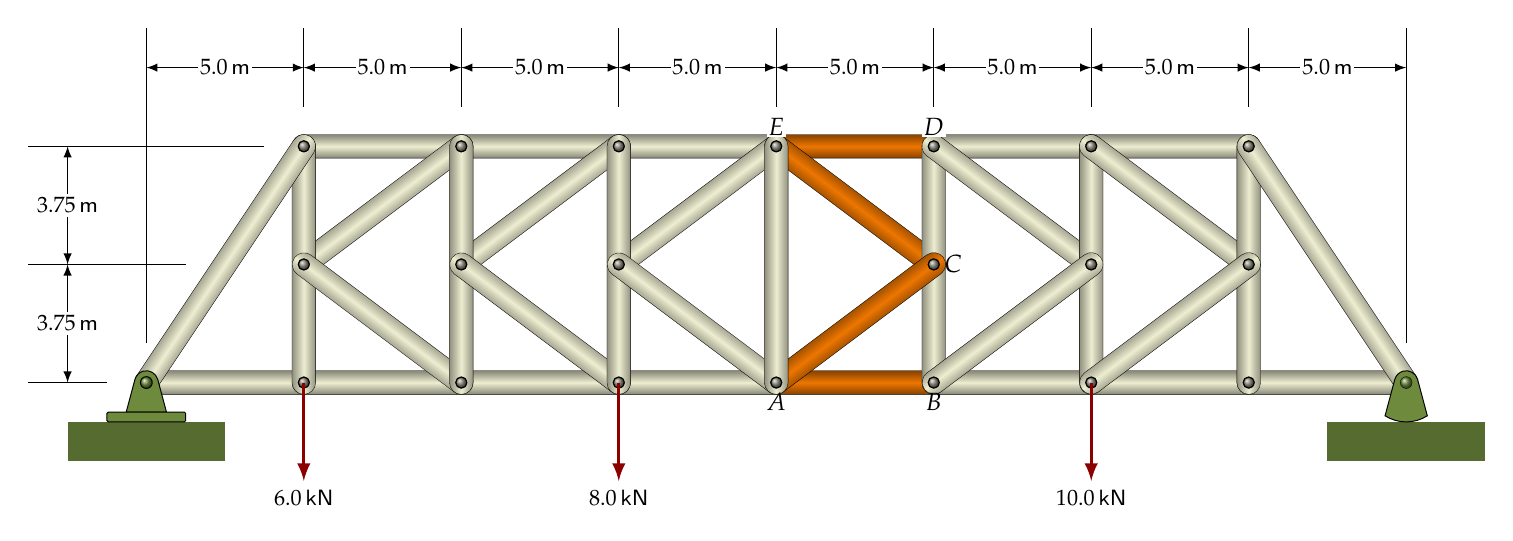
\begin{tikzpicture}[scale=\scale]

	\footnotesize

	\coordinate (A) at (0,0);
	\coordinate (B)	at (2, 0);
	\coordinate (C) at (4,0);
	\coordinate (D) at (6,0);
	\coordinate (E) at (8,0);
	\coordinate (F) at (10,0);
	\coordinate (G) at (12,0);
	\coordinate (H) at (14,0);
	\coordinate (I) at (16,0);
	\coordinate (J) at (18,0);
	\coordinate (Btop) at (2,3);
	\coordinate (Ctop) at (4,3);
	\coordinate (Dtop) at (6,3);
	\coordinate (Etop) at (8,3);
	\coordinate (Ftop) at (10,3);
	\coordinate (Gtop) at (12,3);
	\coordinate (Htop) at (14,3);
	\coordinate (Itop) at (16,3);
	\coordinate (Bmid) at (2,1.5);
	\coordinate (Cmid) at (4,1.5);
	\coordinate (Dmid) at (6,1.5);
	\coordinate (Emid) at (8,1.5);
	\coordinate (Fmid) at (10,1.5);
	\coordinate (Gmid) at (12,1.5);
	\coordinate (Hmid) at (14,1.5);
	\coordinate (Imid) at (16,1.5);

	\Meme{A}{B}{LightYellow4}{LightYellow2}{black}{0.3}{0.15}{0.125}
	\Meme{C}{B}{LightYellow4}{LightYellow2}{black}{0.3}{0.15}{0.125}
	\Meme{C}{D}{LightYellow4}{LightYellow2}{black}{0.3}{0.15}{0.125}
	\Meme{E}{D}{LightYellow4}{LightYellow2}{black}{0.3}{0.15}{0.125}
	\Meme{E}{F}{DarkOrange4}{DarkOrange2}{black}{0.3}{0.15}{0.125}
	\Meme{G}{F}{LightYellow4}{LightYellow2}{black}{0.3}{0.15}{0.125}
	\Meme{G}{H}{LightYellow4}{LightYellow2}{black}{0.3}{0.15}{0.125}
	\Meme{I}{H}{LightYellow4}{LightYellow2}{black}{0.3}{0.15}{0.125}
	\Meme{Gtop}{Htop}{LightYellow4}{LightYellow2}{black}{0.3}{0.15}{0.125}
	\Meme{Gtop}{Ftop}{LightYellow4}{LightYellow2}{black}{0.3}{0.15}{0.125}
	\Meme{Etop}{Ftop}{DarkOrange4}{DarkOrange2}{black}{0.3}{0.15}{0.125}
	\Meme{Etop}{Dtop}{LightYellow4}{LightYellow2}{black}{0.3}{0.15}{0.125}
	\Meme{Ctop}{Dtop}{LightYellow4}{LightYellow2}{black}{0.3}{0.15}{0.125}
	\Meme{Ctop}{Btop}{LightYellow4}{LightYellow2}{black}{0.3}{0.15}{0.125}

	\Meme{Ctop}{Bmid}{LightYellow4}{LightYellow2}{black}{0.3}{0.15}{0.125}
	\Meme{Btop}{B}{LightYellow4}{LightYellow2}{black}{0.3}{0.15}{0.125}
	\Meme{C}{Bmid}{LightYellow4}{LightYellow2}{black}{0.3}{0.15}{0.125}
	
	\Meme{Dtop}{Cmid}{LightYellow4}{LightYellow2}{black}{0.3}{0.15}{0.125}
	\Meme{Ctop}{C}{LightYellow4}{LightYellow2}{black}{0.3}{0.15}{0.125}
	\Meme{D}{Cmid}{LightYellow4}{LightYellow2}{black}{0.3}{0.15}{0.125}

	\Meme{Etop}{Dmid}{LightYellow4}{LightYellow2}{black}{0.3}{0.15}{0.125}
	\Meme{Dtop}{D}{LightYellow4}{LightYellow2}{black}{0.3}{0.15}{0.125}
	\Meme{E}{Dmid}{LightYellow4}{LightYellow2}{black}{0.3}{0.15}{0.125}

	\Meme{Etop}{Fmid}{DarkOrange4}{DarkOrange2}{black}{0.3}{0.15}{0.125}	
	\Meme{Ftop}{F}{LightYellow4}{LightYellow2}{black}{0.3}{0.15}{0.125}
	\Meme{Fmid}{E}{DarkOrange4}{DarkOrange2}{black}{0.3}{0.15}{0.125}

	\Meme{Ftop}{Gmid}{LightYellow4}{LightYellow2}{black}{0.3}{0.15}{0.125}	
	\Meme{Gtop}{G}{LightYellow4}{LightYellow2}{black}{0.3}{0.15}{0.125}
	\Meme{Gmid}{F}{LightYellow4}{LightYellow2}{black}{0.3}{0.15}{0.125}

	\Meme{Gtop}{Hmid}{LightYellow4}{LightYellow2}{black}{0.3}{0.15}{0.125}	
	\Meme{Htop}{H}{LightYellow4}{LightYellow2}{black}{0.3}{0.15}{0.125}
	\Meme{Hmid}{G}{LightYellow4}{LightYellow2}{black}{0.3}{0.15}{0.125}

	\Meme{Etop}{E}{LightYellow4}{LightYellow2}{black}{0.3}{0.15}{0.125}
	\Meme{Htop}{I}{LightYellow4}{LightYellow2}{black}{0.3}{0.15}{0.125}
	\Meme{Btop}{A}{LightYellow4}{LightYellow2}{black}{0.3}{0.15}{0.125}

	\foreach \coord in {A,B,...,I, Bmid, Cmid,Dmid, Fmid, Gmid, Hmid, Btop, Ctop, Dtop, Etop, Ftop, Gtop, Htop}{
		\filldraw[ball color = LightYellow4] (\coord) circle (2pt);
	};
	\foreach \coord in {Btop, Ctop, Dtop, Etop, Ftop, Gtop, Htop}{
		\draw ($(\coord)+(0,0.5)$) -- +(0,1);
	};
	\draw ($(A)+(0,0.5)$) -- +(0,4);
	\draw ($(I)+(0,0.5)$) -- +(0,4);
	\draw ($(Btop)+(-0.5,0)$) -- +(-3,0);
	\draw ($(A)+(-0.5,0)$) -- +(-1,0);
	\draw ($(Bmid)+(-1.5,0)$) -- +(-2,0);

	\foreach \x in {0, 1, ..., 7}{
		\draw[latex-latex] (2*\x, 4) -- +(2,0)node[fill=white, midway, inner sep = 0.25mm]{\footnotesize $ 5.0\,\textsf{m} $};
	}

	\draw[latex-latex] (-1,3) -- (-1,1.5)node[fill=white, midway, inner sep = 0.5mm]{\footnotesize $ 3.75\,\textsf{m} $};
	\draw[latex-latex] (-1,1.5) -- (-1,0)node[fill=white, midway, inner sep = 0.5mm]{\footnotesize $ 3.75\,\textsf{m} $};

	\fill[DarkOliveGreen] ($(A)+(-1,-0.5)$) rectangle +(2,-0.5);
	\fill[DarkOliveGreen] ($(I)+(-1,-0.5)$) rectangle +(2,-0.5);
	\PC{A}{DarkOliveGreen4}{black}{0.5}{0.125}
	\Rocker{I}{DarkOliveGreen4}{black}{0.5}{0.125}

	\draw[very thick, -latex, statsMaroon] (B)--+(0,-1.25)node[below, black]{$ 6.0\,\textsf{kN}$ };
	\draw[very thick, -latex, statsMaroon] (D)--+(0,-1.25)node[below, black]{$ 8.0\,\textsf{kN}$ };
	\draw[very thick, -latex, statsMaroon] (G)--+(0,-1.25)node[below, black]{$ 10.0\,\textsf{kN}$ };

	\small
	\node[yshift=-0.25cm] at (E) {$ A $};
	\node[yshift=-0.25cm] at (F) {$ B $};
	\node[yshift=0.25cm, fill=white, inner sep = 0.2mm] at (Ftop) {$ D $};
	\node[yshift=0.25cm, fill=white, inner sep = 0.2mm] at (Etop) {$ E $};
	\node[xshift=0.25cm,] at (Fmid) {$ C $};
	
\end{tikzpicture}

		\pars
		Use the method of sections to determine the internal forces in members $EF$, $EQ$, $LM$ and $MQ$.
		\pars
	\end{myexam}
\end{frame}

%%%%%%%%%%%%%%%%%%%%%%%%%%%%%%%%%%%%%%%%%%%%%%%%%%%%%%%%%%%%%%%%%%%%%%%%%%%%%%%%%%%%%%%%%%%%%%%%%%%%
\begin{frame}{}
	\def\scale{0.575}
	
	\begin{myexer}{}{}		
			\centering
			\input{../../pikz/08MoS/08MoS03.tex}
			\parb		
			Determine the forces in members $CF$, $CG$,$EG$ and $EH$.
			\parb		
		
	\end{myexer}

\end{frame}

%


%%%%%%%%%%%%%%%%%%%%%%%%%%%%%%%%%%%%%%%%%%%%%%%%%%%%%%%%%%%%%%%%%%%%%%%%%%%%%%%%

\end{document}